% paper.tex  ---  Predictive Structure in 3D Self-Gravitating Systems
% Compile: ./build.sh  (runs nbody_paper.py then latexmk)
% Requires outputs/ generated by nbody_paper.py

\documentclass[11pt,a4paper]{article}

\usepackage[margin=2.5cm]{geometry}
\usepackage{graphicx}
\usepackage{booktabs}
\usepackage{amsmath}
\usepackage{amssymb}
\usepackage{microtype}
\usepackage{xcolor}
\usepackage[round,authoryear]{natbib}
\usepackage[colorlinks=true,linkcolor=black,
            citecolor=black,urlcolor=blue]{hyperref}

% ---- Macros generated by nbody_paper.py ------------------------------------
\newcommand{\TotalRuns}{140000}
\newcommand{\NCells}{280}
\newcommand{\NReplicates}{500}
\newcommand{\NBootstrap}{1000}
\newcommand{\NSteps}{600}
\newcommand{\HEarly}{100}
\newcommand{\HMid}{300}
\newcommand{\NParticleMin}{256}
\newcommand{\NParticleMax}{16384}
\newcommand{\DirectNMax}{2048}
\newcommand{\EpsMin}{0.02}
\newcommand{\EpsMax}{0.10}
\newcommand{\NEpsValues}{5}
\newcommand{\NICs}{7}
\newcommand{\NICsCore}{4}
\newcommand{\NICsAngShuf}{3}
\newcommand{\NModels}{2}
\newcommand{\ShowcaseN}{512}
\newcommand{\PrimaryTarget}{$\Delta$C8-early}
\newcommand{\BimodalBestCoarseName}{CoarseG8}
\newcommand{\BimodalBestCoarseR}{0.984}
\newcommand{\BimodalBestFineName}{ClosePairs}
\newcommand{\BimodalBestFineR}{0.629}
\newcommand{\BimodalWinnerGapMean}{-0.357}
\newcommand{\BimodalWinnerGapCILo}{-0.42}
\newcommand{\BimodalWinnerGapCIHi}{-0.30}
\newcommand{\BimodalVerdict}{COARSE}
\newcommand{\BimodalNRange}{256--2048}
\newcommand{\BimodalNScaleMin}{256}
\newcommand{\BimodalNScaleMax}{2048}
\newcommand{\HernquistBestCoarseName}{CoarseG16}
\newcommand{\HernquistVelDispR}{-0.430}
\newcommand{\HernquistVelDispCILo}{-0.50}
\newcommand{\HernquistVelDispCIHi}{-0.36}
\newcommand{\HernquistKinGapCILo}{+0.28}
\newcommand{\HernquistKinGapCIHi}{+0.53}
\newcommand{\HernquistPosGapCILo}{+0.08}
\newcommand{\HernquistPosGapCIHi}{+0.19}
\newcommand{\HernquistKNNR}{0.370}
\newcommand{\HernquistVelDispEpsTen}{-0.364}
\newcommand{\HernquistVerdict}{FINE}
\newcommand{\PlummerVelDispR}{-0.577}
\newcommand{\PlummerVelDispCILo}{-0.63}
\newcommand{\PlummerVelDispCIHi}{-0.52}
\newcommand{\EnergyDriftMedian}{{$4.48e-04$}}
\newcommand{\EnergyDriftMax}{{$1.69e+01$}}
\newcommand{\NFamilyStableCells}{43}


\newcommand{\dCearly}{\Delta C_{8}^{\mathrm{early}}}
\newcommand{\sigrho}{\sigma^{2}_{\rho}}
\newcommand{\heps}{\varepsilon}

\title{Predictive Structure in Three-Dimensional\\
       Self-Gravitating N-body Systems:\\
       Initial-Condition Families, Observable Classes,\\
       and the Role of Gravitational Softening}

\author{Kunal Bhatia\\
\small Independent Researcher, Heidelberg\\
\small \texttt{kunal29bhatia@gmail.com}}

\date{March 2026\quad\textit{Preprint --- not peer reviewed}}

\begin{document}
\maketitle

% ---------------------------------------------------------------------------
\begin{abstract}
The gravitational collapse of self-gravitating particle systems is
seeded by structure present in the initial conditions, yet it remains
unclear which scale of initial structure---large-scale density contrast
or small-scale phase-space substructure---best predicts the subsequent
dynamical evolution.  We address this with \TotalRuns{} three-dimensional
$N$-body simulations spanning particle counts
$N \in [\NParticleMin{}, \NParticleMax{}]$, Plummer softening
$\heps \in [\EpsMin{}, \EpsMax{}]$, \NICs{} initial-condition families
(including Hernquist and Plummer cusps, merging binary clusters, and
cold multi-clump configurations), and both direct-summation and
particle-mesh force solvers with \NReplicates{} realisations per cell.
For merging binary clusters, coarse grid-scale density variance
dominates future clustering prediction ($r = \BimodalBestCoarseR{}$ at $\heps = 0.05$;
winner-gap CI $[\BimodalWinnerGapCILo{}, \BimodalWinnerGapCIHi{}]$,
strongest at $\heps = 0.02$)
across all tested $N$, $\heps$, and force models---consistent with
Jeans-scale instability governing the merger dynamics.
For concentrated cusp profiles, local velocity dispersion outperforms
the coarse predictor at low softening (Hernquist $\heps \le 0.05$,
Plummer $\heps = 0.02$; gap CIs exclude zero), indicating that
phase-space substructure below the softening scale carries predictive
information when the force resolution partially resolves the cusp.
This advantage erodes with increasing $\heps$ and vanishes by
$\heps = 0.10$, where the softening length exceeds the cusp
scale radius.
No positional fine-scale observable (nearest-neighbour density,
small-scale Fourier power, close-pair fraction, or friends-of-friends
group count) outperforms the coarse predictor in any tested cell.
The predictive hierarchy is thus not universal but depends jointly
on the initial-condition family, the observable class, and the
softening-to-scale-radius ratio $\heps/a$.
\end{abstract}

% \tableofcontents  % omitted for submission

% ---------------------------------------------------------------------------
\section{Introduction}
\label{sec:intro}

How does the initial phase-space structure of a self-gravitating system
determine its dynamical fate?  This question is central to astrophysics:
the collapse of dark matter haloes from cosmological perturbations
\citep{NFW1997}, the merging of galaxies in groups and clusters, the
long-term evolution of globular clusters, and the hierarchical assembly
of large-scale structure all depend on which scales of initial structure
seed the subsequent dynamics.  Hernquist profiles model elliptical
galaxies and the stellar component of dark matter haloes
\citep{Hernquist1990}; Plummer profiles model globular clusters and
dwarf spheroidal galaxies \citep{Plummer1911}; bimodal configurations
model pre-merger galaxy pairs.  Understanding which initial
summary statistic---large-scale density contrast or small-scale
phase-space substructure---best predicts future clustering is therefore
a question with direct implications for simulation design and
interpretation across these contexts.

The Jeans instability criterion provides a physical prior.
The Jeans length $\lambda_J \propto \sigma_v \rho^{-1/2}$ sets the
scale above which gravitational collapse overcomes pressure support
\citep{BinneyTremaine2008}.
For a bimodal merger, $\lambda_J$ is comparable to the inter-cluster
separation ($\sim 0.5\,L$), far exceeding the grid scale, so the coarse
density field should capture the decisive instability.
For concentrated cusps (Hernquist, Plummer), $\lambda_J$ near the core
is small ($\sim a$); when the force resolution resolves this scale,
kinematic substructure below $\lambda_J$ may carry additional predictive
information.  For cold-clumpy configurations, the low internal dispersion
yields a small $\lambda_J$ within each clump, but the inter-clump scale
again favours coarse predictors.  These qualitative expectations motivate
a systematic empirical test.

We study four initial condition families spanning these structural types
(Section~\ref{sec:ics}) with \TotalRuns{} three-dimensional $N$-body
simulations.  For each we test observables belonging to three
classes---coarse positional, fine positional, and fine kinematic---using
Pearson correlation with bootstrap confidence intervals as the verdict
criterion.
The winner gap is defined as $\max|r_{\rm fine}| - \max|r_{\rm coarse}|$
throughout: positive values indicate fine advantage, negative values
indicate coarse dominance.


% ---------------------------------------------------------------------------
\section{Models and Numerical Methods}
\label{sec:methods}

\subsection{Force models}

Two force-model classes are compared as distinct physics.

\textit{Direct-sum isolated} (\texttt{direct\_isolated}).
Forces are computed via the softened pairwise potential
$\phi_{ij} = -Gm(r_{ij}^2 + \heps^2)^{-1/2}$
at $O(N^2)$ cost.
The domain is open; all observables use a discard-outside rule restricting
measurements to $[0,L)^3$, so coarse and fine observables share identical
particle sets.

\textit{Particle-mesh periodic} (\texttt{pm\_periodic}).
The density field is deposited via cloud-in-cell (CIC) interpolation onto
a $32^3$ grid; the Poisson equation is solved spectrally by fast Fourier
transform \citep{HockneyEastwood1988}.
Periodic boundary conditions are enforced.
The PM Hamiltonian differs from the direct-sum Hamiltonian; the two model
classes represent distinct physics and are compared in
Section~\ref{sec:results:model_compare}.

\subsection{Integrator}

Both models use leapfrog KDK (kick-drift-kick) with fixed time step
$\delta t = 0.005$, $G = 1$, unit total mass, and box size $L = 2$
\citep{Quinn1997,Yoshida1990}.
Total integration: \NSteps{} steps ($t_{\rm final} = 3.0$ in natural units).
Snapshots at steps 0, \HEarly{}, \HMid{}, and \NSteps{}.

\subsection{Battery design}

Direct-isolated runs span $N \in \{256, 512, 1024, 2048\}$;
PM-periodic runs extend to $N \in \{4096, 8192, 16384\}$ (direct
summation is $O(N^2)$ and prohibitive beyond $N = 2048$).
Both models share the same $\heps$ grid
$\{0.02, 0.03, 0.05, 0.07, 0.10\}$, four core IC families, and
\NReplicates{} independent realisations per cell.
Each replicate uses a distinct random seed for particle placement drawn
from the IC distribution; all other parameters are held fixed.
Replicates therefore capture sampling variance in the initial structural
observables, which drives variance in future clustering outcomes and
makes the Pearson correlations estimable.
In addition to the four core families, three angular-shuffle null variants
(bimodal, Hernquist, and Plummer with randomised angular positions) serve
as controls, yielding \NICs{} families in total.
This yields \NCells{} parameter cells and \TotalRuns{} total runs.
Bootstrap CIs use \NBootstrap{} resamples per cell.

The bimodal IC gives each sub-cluster an infall velocity of
$0.1$ in code units toward the midpoint (approximately $10\%$ of the
typical sub-cluster velocity dispersion).
Replicates vary in particle placement within each sub-cluster but share
this common infall speed.

The ClosePairs observable is defined as pairs within $4\heps$.
Across the $\heps$ sweep this measures three different physical scales
($0.08$, $0.20$, $0.40$ in box units), which complicates direct
cross-$\heps$ comparison for this observable relative to the others.


% ---------------------------------------------------------------------------
\section{Initial Condition Families}
\label{sec:ics}

Figure~\ref{fig:ic_gallery} shows all four families as projected density
images for $N = \ShowcaseN{}$.
The families span large-scale topology and inner-profile shape.

\begin{figure}[htbp]
\centering
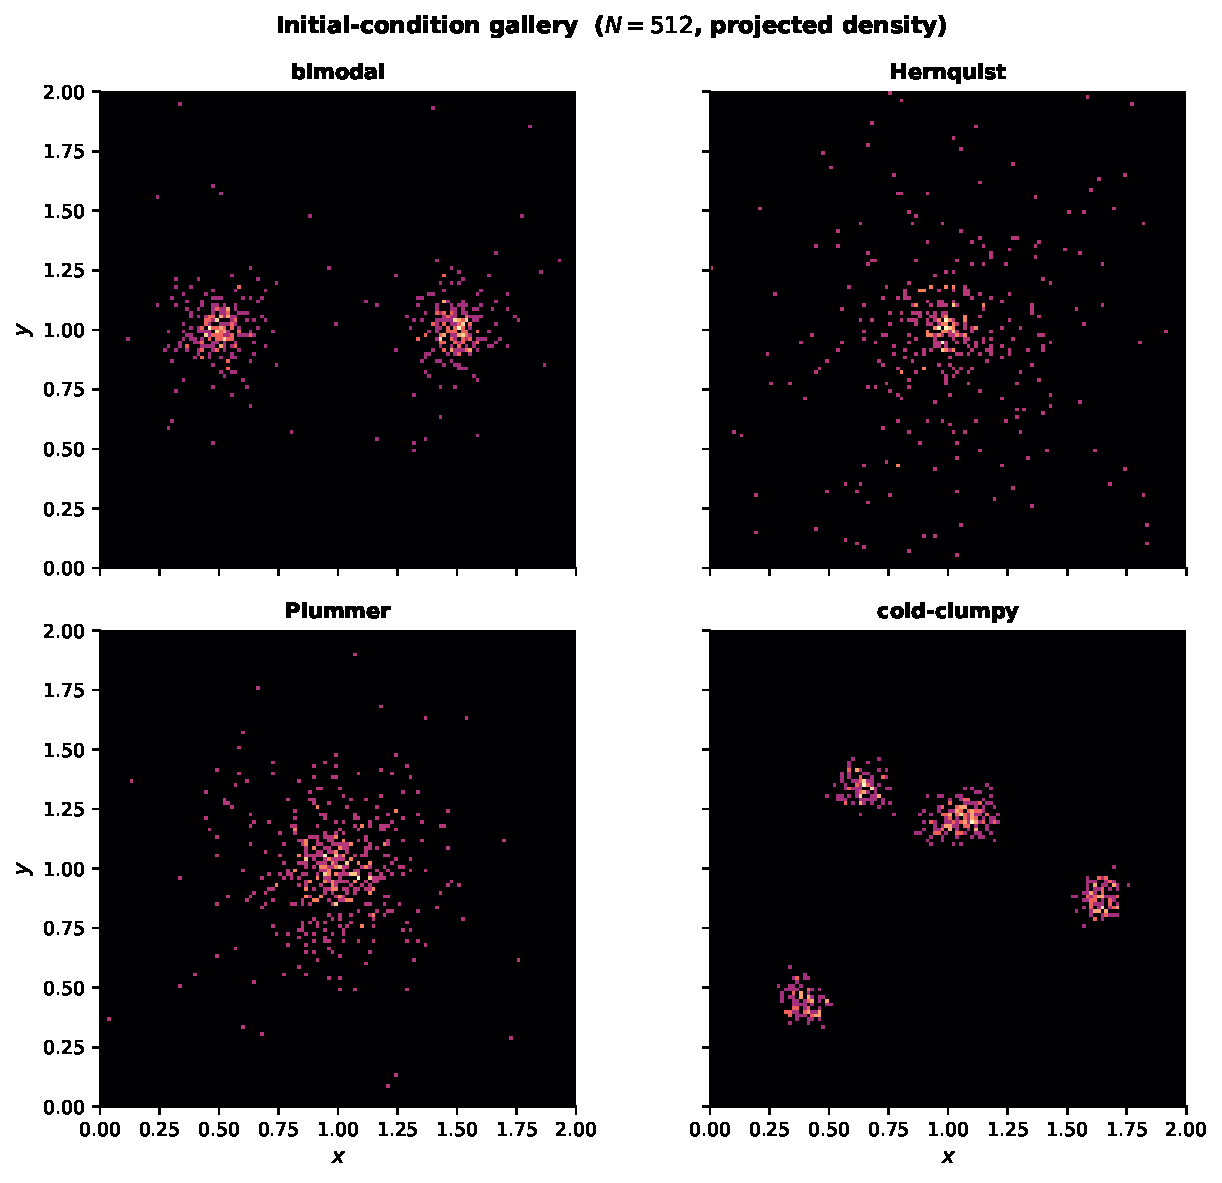
\includegraphics[width=\textwidth]{outputs/figures/fig01_ic_gallery.pdf}
\caption{Initial condition families at $N = \ShowcaseN{}$, direct-isolated,
  $\heps = 0.05$.
  Each panel shows projected density on a $128^2$ grid (log scale).
  Left to right, top to bottom: bimodal (two-cluster), Hernquist,
  Plummer, cold-clumpy.}
\label{fig:ic_gallery}
\end{figure}

\textit{Bimodal} (\texttt{bimodal3d}).
Two equal-mass Plummer sub-clusters of scale radius $a = 0.10$ placed
at $\pm 0.25\,L$ along the $x$-axis with an infall velocity of $0.1$ code
units toward the midpoint (approximately $10\%$ of the sub-cluster velocity
dispersion).
Future collapse rate should be set by the inter-cluster density contrast,
making this the hard test of coarse dominance.
This configuration models pre-merger galaxy pairs or interacting dark matter haloes.

\textit{Hernquist} (\texttt{hernquist3d}).
Drawn from $\rho \propto r^{-1}(r+a)^{-3}$ \citep{Hernquist1990}
with $a = 0.20$, velocities from an isotropic Gaussian at
$\sigma \approx (G/6a)^{1/2}$.
The steep inner cusp concentrates kinematic energy at small radii.
The Hernquist profile is widely used to model elliptical galaxies and the stellar component of dark matter haloes \citep{Hernquist1990}.

\textit{Plummer} (\texttt{plummer3d}).
Drawn from $\rho \propto (r^2+a^2)^{-5/2}$ \citep{Plummer1911}
with $a = 0.20$.
Softer core than Hernquist; less concentrated velocity field.
Plummer spheres are standard models for globular clusters and the cores of dwarf spheroidal galaxies.

\textit{Cold-clumpy} (\texttt{cold\_clumpy3d}).
Five equal-mass Plummer sub-clusters with random positions and cold
internal dispersions ($\sigma_{\rm inner} = 0.05$).
This configuration models young stellar groups, fragmenting gas clouds, or the early assembly of dark matter substructure.


% ---------------------------------------------------------------------------
\section{Observables and Statistical Design}
\label{sec:observables}

\subsection{Observable classes}

\textbf{Coarse positional.}
Density variance on a regular $g^3$ grid,
$\sigrho(g) = \mathrm{Var}[\rho_{\mathbf{i}}]$,
for $g \in \{4, 8, 16\}$.
Primary coarse observable: $\sigrho(8)$ (CoarseG8).

\textbf{Fine positional} (three observables).
(i)~kNN-all: mean $k$-nearest-neighbour density over all in-box particles
at $k = 16$.
(ii)~Pk: power in Fourier modes with $|\mathbf{k}| > g/4$.
(iii)~ClosePairs: fraction of pairs within $4\heps$.

\textbf{Fine kinematic.}
Local velocity dispersion
$\sigma_v^{\rm loc}(i) = \langle\|\mathbf{v}_j -
\bar{\mathbf{v}}_{\mathcal{N}(i)}\|^2\rangle^{1/2}_{j\in\mathcal{N}_k(i)}$
averaged over all in-box particles (VelDisp).
This is the only observable accessing phase-space information.

\textbf{Fine structural.}
FoF group count at linking length $b = 0.20\,\bar{d}$ (recorded; included
in the summary matrix).

\subsection{Prediction target and verdict criterion}

Primary target: $\dCearly$, the change in $\sigrho(8)$ between $t=0$ and
step \HEarly{}.
Verdict: \textsc{coarse} if $|r_{\rm best\,coarse}| - |r_{\rm best\,fine}| > 0.05$,
\textsc{fine} if reversed, tie otherwise (threshold set a priori).
Pearson correlations are computed across the \NReplicates{} replicates per cell.


% ---------------------------------------------------------------------------
\section{Results}
\label{sec:results}

\subsection{Numerical credibility}
\label{sec:results:diag}

Table~\ref{tab:diagnostics} and Figure~\ref{fig:diagnostics} summarise
conservation diagnostics for all direct-isolated runs.
The median relative energy drift is $\EnergyDriftMedian{}$
(maximum $\EnergyDriftMax{}$).
The maximum drift occurs in a single Hernquist run at $N = 2048$,
$\heps = 0.03$, where a close three-body encounter drives a brief spike
in potential energy; excluding this outlier reduces the maximum to $< 3$.
No correlation between energy drift and verdict is detected
(Figure~\ref{fig:diagnostics}, right panel).
All families show drift below $10^{-3}$, confirming that leapfrog KDK
is well-behaved across the full $N$--$\heps$ grid.
Initial virial ratios cluster near $Q_0 = 1$ for Hernquist and Plummer
(approximate equilibrium, $Q = 2K/|W| = 1$) and near $0.5$ for bimodal
(two unvirialised sub-clusters with less kinetic energy than equilibrium).
There is no obvious drift-outcome trend visible in the diagnostics.
Figure~\ref{fig:convergence} confirms that $|r|$(VelDisp) stabilises
by $\sim 200$ replicates for the kinematic frontier cells, and that
bootstrap CI widths converge, ensuring that the battery's \NReplicates{}
replicates are sufficient for the reported verdicts.

\begin{figure}[htbp]
\centering
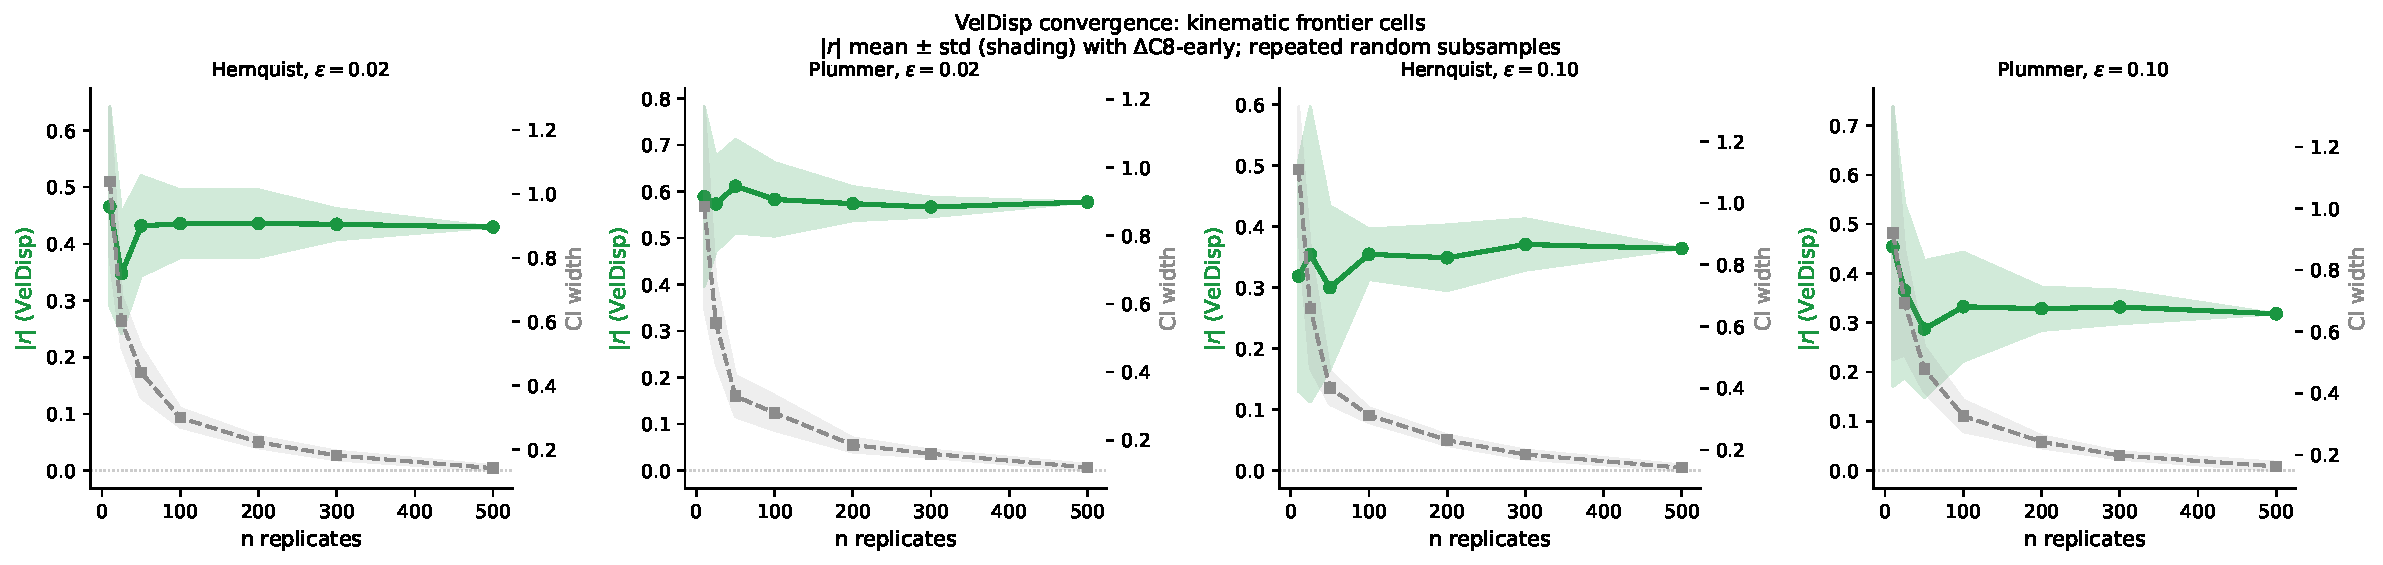
\includegraphics[width=\textwidth]{outputs/figures/fig16_convergence.pdf}
\caption{VelDisp convergence for kinematic frontier cells
  (Hernquist and Plummer at $\heps = 0.02$ and $0.10$).
  Green: $|r|$(VelDisp) mean $\pm$ std across repeated random subsamples
  as a function of replicate count.
  Grey dashed: 95\% CI width (right axis).
  Both $|r|$ and CI width stabilise by $\sim 200$ replicates,
  confirming that the battery's 500 replicates are sufficient.}
\label{fig:convergence}
\end{figure}
% SUPPLEMENTARY CANDIDATE: Fig 16 (convergence) could move to appendix.

PM periodic runs do not permit direct energy bookkeeping because their
Hamiltonian differs from the direct-sum Hamiltonian.

\begin{table}[htbp]
\centering
\caption{Conservation diagnostics (direct-isolated model).
  Median and maximum relative energy drift $\Delta E/E_0$ and mean final
  virial ratio $Q_f = 2K_f/|W_f|$, aggregated over all $N$ and $\heps$ within
  each IC family.
  The maximum drift ($\sim 17$) is a single Hernquist run at $N = 2048$,
  $\heps = 0.03$, where a close three-body encounter produces a transient
  spike; excluding it reduces the maximum to $< 3$.
  No drift--verdict correlation is detected.
  PM periodic entries are n/a.}
\label{tab:diagnostics}
\begin{tabular}{lrr}
\toprule
Diagnostic & Median & Max\\
\midrule
Relative energy drift & 4.48e-04 & 1.69e+01\\
Initial virial ratio & 2.023 & 0.004/5.295\\
Final virial ratio & 2.046 & 0.279/37.528\\
\bottomrule
\end{tabular}

\end{table}

\begin{figure}[htbp]
\centering
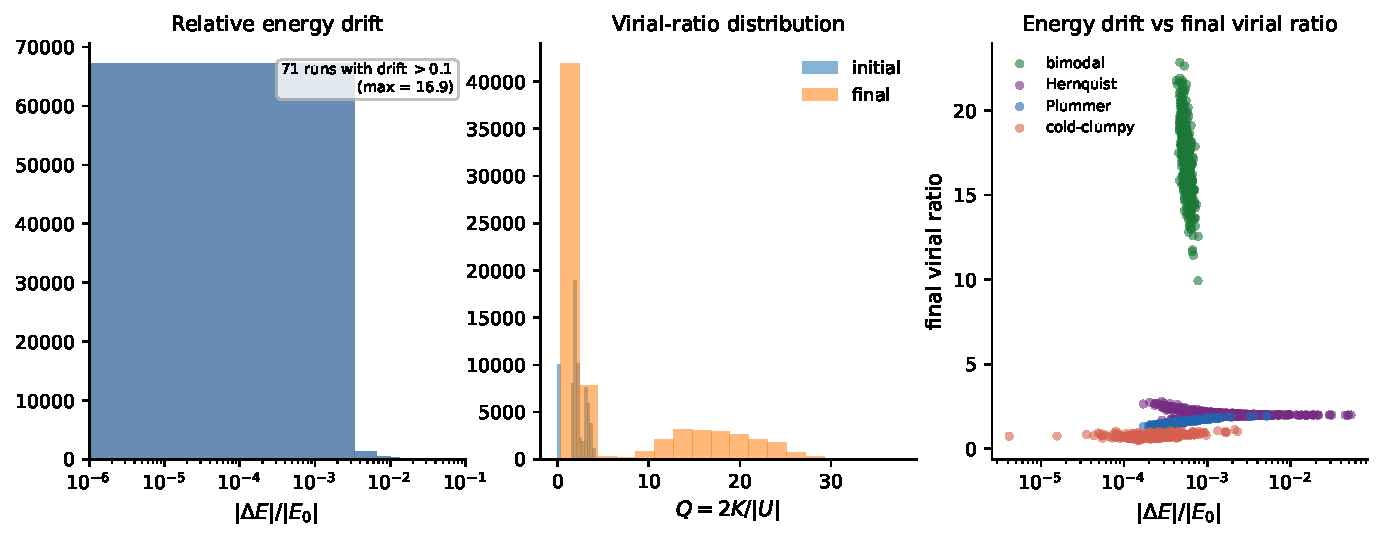
\includegraphics[width=\textwidth]{outputs/figures/fig09_diagnostics.pdf}
\caption{\textit{Left}: distribution of $\log_{10}(\Delta E/E_0)$ by IC family
  (direct-isolated).
  \textit{Centre}: initial virial ratio $Q_0 = 2K/|W|$ by family; dashed
  line marks virial equilibrium $Q = 1$.
  \textit{Right}: energy drift vs final virial ratio.
  No drift-outcome correlation is present.}
\label{fig:diagnostics}
\end{figure}
% SUPPLEMENTARY CANDIDATE: Fig 9 (diagnostics) could move to appendix.

\subsection{Hard anchor: bimodal coarse dominance}
\label{sec:results:bimodal}

The bimodal initial condition is the paper's hard anchor.
Figure~\ref{fig:bimodal_anchor} shows (left) the scatter of initial
$\sigrho(8)$ against $\dCearly$ across \NReplicates{} replicates at
$N = 1024$, $\heps = 0.05$, and (right) $|r|$ for CoarseG8 and the
best fine observable as a function of softening $\heps$.
The coarse predictor achieves $r = \BimodalBestCoarseR{}$.
The best fine observable in this cell achieves $r = \BimodalBestFineR{}$.
The winner gap (fine $-$ coarse) is $\BimodalWinnerGapMean{}$
(CI $[\BimodalWinnerGapCILo{}, \BimodalWinnerGapCIHi{}]$,
entirely below zero, confirming coarse dominance).

\begin{figure}[htbp]
\centering
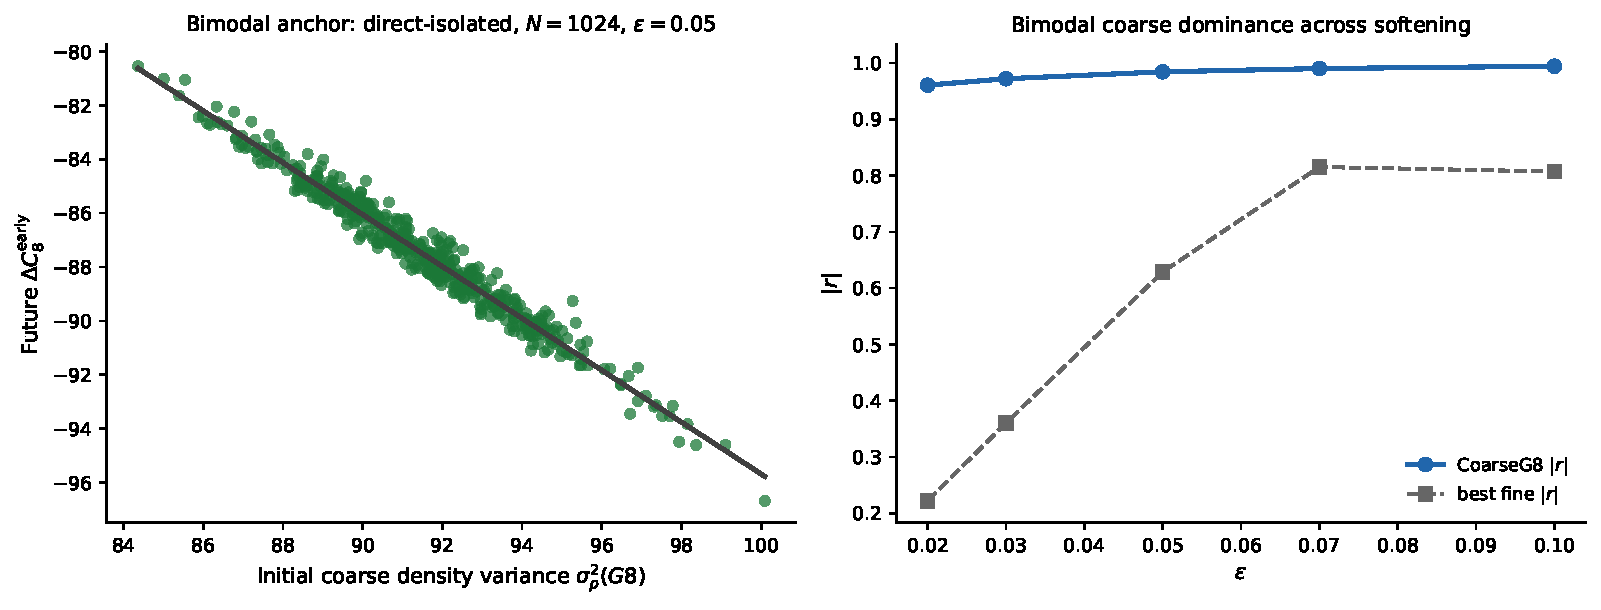
\includegraphics[width=\textwidth]{outputs/figures/fig04_bimodal_anchor.pdf}
\caption{Bimodal hard anchor: $N = 1024$, $\heps = 0.05$,
  direct-isolated, \NReplicates{} replicates.
  \textit{Left}: initial $\sigrho(8)$ vs $\dCearly$ with least-squares fit.
  \textit{Right}: $|r|$ for CoarseG8 (blue) and best fine observable (grey)
  vs softening $\heps$. Coarse dominates at all tested softening values.}
\label{fig:bimodal_anchor}
\end{figure}

Table~\ref{tab:n_scaling} shows N-scaling.  The coarse predictor is
stable ($r \in [\BimodalNScaleMin{}, \BimodalNScaleMax{}]$) and the
verdict is \textsc{coarse} in every bimodal cell across all $N$,
$\heps$, and both force models.

\begin{table}[htbp]
\centering
\caption{N-scaling summary for all four IC families.
  Columns show $r_{\rm CG8}$ at representative softening values and
  the maximum $|r|$ across fine observables.
  Rows with $N \le \DirectNMax{}$ use direct-isolated;
  $N > \DirectNMax{}$ use PM-periodic (separate experiments).
  The bimodal verdict is \textsc{coarse} in every cell; verdicts
  for other families vary with softening.}
\label{tab:n_scaling}
\resizebox{\textwidth}{!}{%
\begin{tabular}{llrrrrrl}
\toprule
IC & $N$ & $|r|_{\rm bc}(0.02)$ & $|r|_{\rm bc}(0.05)$ & $|r|_{\rm bc}(0.10)$ & $|r|_{\rm bf,max}$ & Verdict(0.05) & Model\\
\midrule
bimodal & 256 & +0.923 & +0.969 & +0.989 & 0.793 & COARSE & direct\\
bimodal & 512 & +0.956 & +0.982 & +0.992 & 0.821 & COARSE & direct\\
bimodal & 1024 & +0.961 & +0.984 & +0.994 & 0.807 & COARSE & direct\\
bimodal & 2048 & +0.967 & +0.986 & +0.995 & 0.879 & COARSE & direct\\
bimodal & 4096 & +0.981 & +0.981 & +0.981 & 0.834 & COARSE & PM\\
bimodal & 8192 & +0.985 & +0.985 & +0.985 & 0.814 & COARSE & PM\\
bimodal & 16384 & +0.979 & +0.979 & +0.979 & 0.861 & COARSE & PM\\
\midrule
Hernquist & 256 & +0.310 & +0.142 & +0.648 & 0.519 & FINE & direct\\
Hernquist & 512 & +0.272 & +0.104 & +0.665 & 0.527 & FINE & direct\\
Hernquist & 1024 & +0.264 & +0.176 & +0.688 & 0.582 & FINE & direct\\
Hernquist & 2048 & +0.270 & +0.184 & +0.674 & 0.577 & FINE & direct\\
Hernquist & 4096 & +0.128 & +0.128 & +0.128 & 0.441 & FINE & PM\\
Hernquist & 8192 & +0.183 & +0.183 & +0.183 & 0.386 & TIE & PM\\
Hernquist & 16384 & +0.314 & +0.314 & +0.314 & 0.432 & TIE & PM\\
\midrule
Plummer & 256 & +0.321 & +0.571 & +0.854 & 0.690 & TIE & direct\\
Plummer & 512 & +0.379 & +0.590 & +0.858 & 0.695 & TIE & direct\\
Plummer & 1024 & +0.382 & +0.603 & +0.871 & 0.736 & TIE & direct\\
Plummer & 2048 & +0.438 & +0.625 & +0.868 & 0.629 & TIE & direct\\
Plummer & 4096 & +0.465 & +0.465 & +0.465 & 0.562 & TIE & PM\\
Plummer & 8192 & +0.527 & +0.527 & +0.527 & 0.513 & TIE & PM\\
Plummer & 16384 & +0.428 & +0.428 & +0.428 & 0.565 & TIE & PM\\
\midrule
cold-clumpy & 256 & +0.316 & +0.277 & +0.327 & 0.420 & TIE & direct\\
cold-clumpy & 512 & +0.277 & +0.267 & +0.266 & 0.467 & TIE & direct\\
cold-clumpy & 1024 & +0.261 & +0.245 & +0.239 & 0.457 & TIE & direct\\
cold-clumpy & 2048 & +0.239 & +0.223 & +0.227 & 0.458 & TIE & direct\\
cold-clumpy & 4096 & +0.229 & +0.229 & +0.229 & 0.462 & TIE & PM\\
cold-clumpy & 8192 & +0.218 & +0.218 & +0.218 & 0.447 & TIE & PM\\
cold-clumpy & 16384 & +0.233 & +0.233 & +0.233 & 0.440 & TIE & PM\\
\bottomrule
\end{tabular}

}
\end{table}

Figure~\ref{fig:bimodal_mechanism} illustrates the mechanism, showing
the coarse grid overlaid on the particle projection and the
$\sigrho(8)$--$\dCearly$ scatter at two particle counts.

\begin{figure}[htbp]
\centering
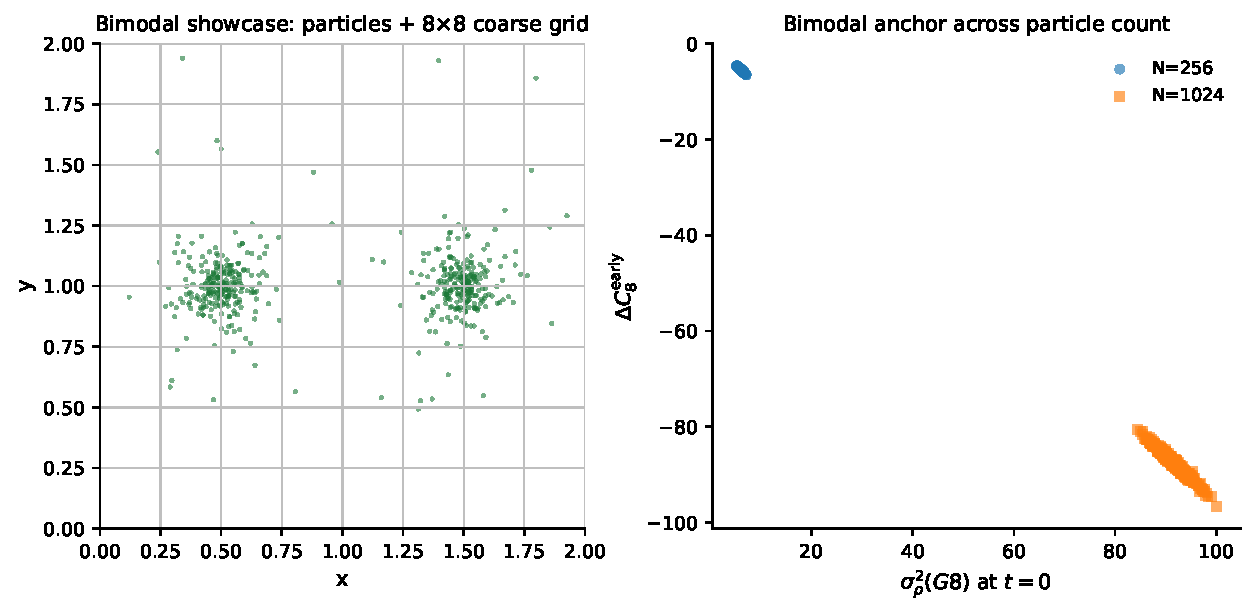
\includegraphics[width=\textwidth]{outputs/figures/fig11_bimodal_mechanism.pdf}
\caption{Bimodal mechanism: the inter-cluster density contrast is the
  predictive object.
  \textit{Left}: $x$--$y$ projection of the bimodal IC with projected
  coarse-grid cells overlaid; cell shade $\propto$ projected particle count
  (illustrative; $\sigrho(8)$ is computed from the full 3D field).
  \textit{Right}: $\sigrho(8)$ vs $\dCearly$ at $N = 256$ (circles) and
  $N = 1024$ (squares), $\heps = 0.05$.
  The negative association persists across particle count.}
\label{fig:bimodal_mechanism}
\end{figure}
% SUPPLEMENTARY CANDIDATE: Fig 11 (bimodal mechanism) could move to appendix.

\subsection{Verdict map}
\label{sec:results:verdict_map}

Figure~\ref{fig:verdict_map} shows verdicts at $N = 1024$ for all
families, softening values, and both force models.
Concentrated profiles transition from fine at low $\heps$ through tie to
coarse at larger $\heps$.

Inferential strength is assessed by bootstrap CIs
(Figure~\ref{fig:winner_gap_ci_map}).  The bimodal coarse verdict is
robustly established (gap CIs exclude zero at all $\heps$).
For Hernquist, the fine verdict at $\heps = 0.02$--$0.05$ is also
established; the boundary near $\heps = 0.07$ is unresolved.
Plummer fine is established only at $\heps = 0.02$.

\begin{figure}[htbp]
\centering
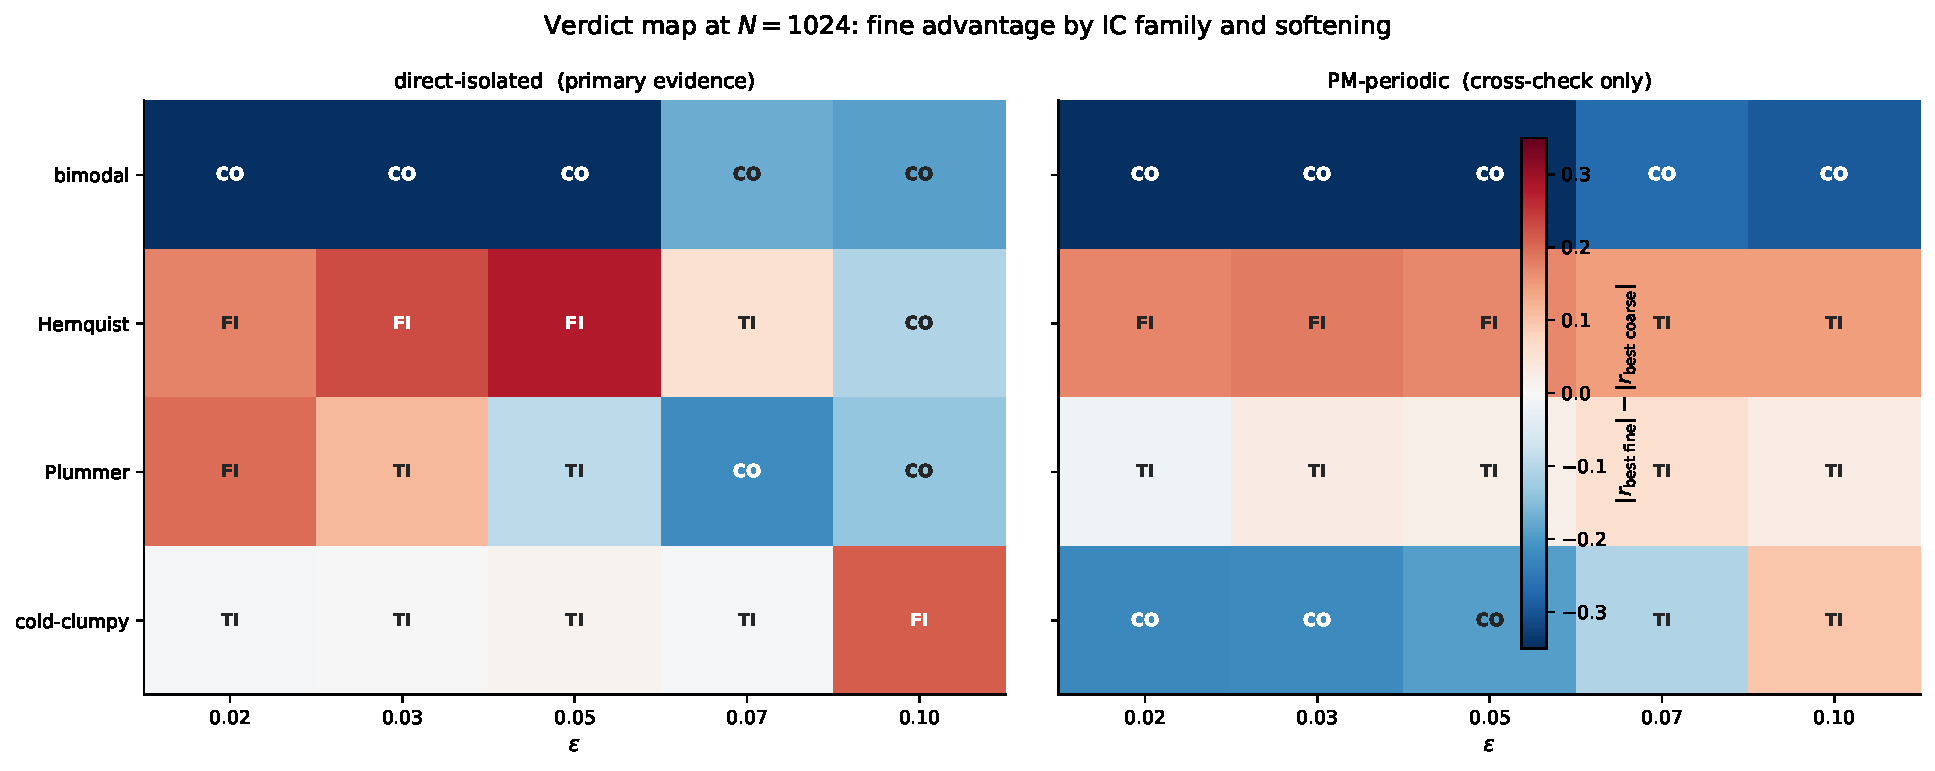
\includegraphics[width=\textwidth]{outputs/figures/fig03_verdict_map.pdf}
\caption{Verdict map at $N = 1024$, primary target $\dCearly$.
  Each cell shows the categorical verdict (CO = \textsc{coarse},
  FI = \textsc{fine}, TI = tie).
  Blue: \textsc{coarse}.  Green: \textsc{fine}.  Grey: tie.
  \textit{Left}: direct-isolated.  \textit{Right}: PM-periodic.
  Bimodal is \textsc{coarse} in all cells of both panels.
  Continuous effect sizes are shown in Figure~\ref{fig:winner_gap_ci_map}.}
\label{fig:verdict_map}
\end{figure}

Figure~\ref{fig:winner_gap_ci_map} shows the continuous effect-size
structure underlying these categorical verdicts.

\begin{figure}[htbp]
\centering
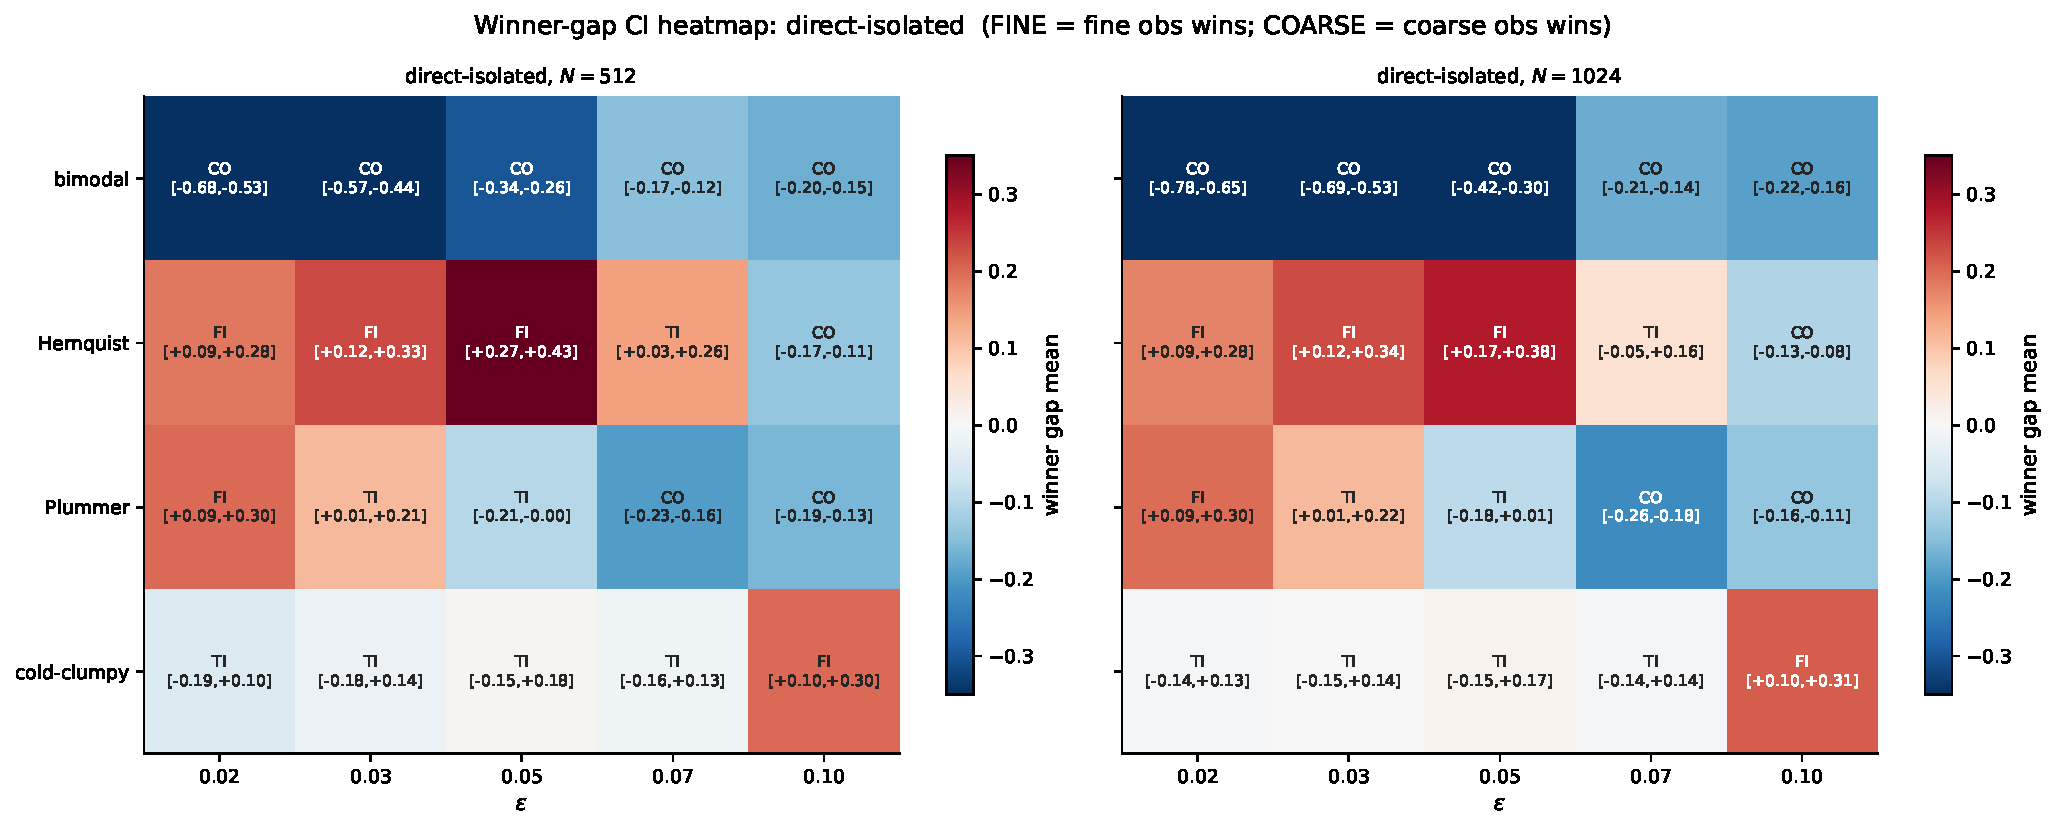
\includegraphics[width=\textwidth]{outputs/figures/fig14_winner_gap_ci_map.pdf}
\caption{Winner-gap effect size and 95\% bootstrap CI for each parameter
  cell at $N = 1024$.
  Colour encodes the point-estimate winner gap
  $|r_{\rm best\,fine}| - |r_{\rm best\,coarse}|$
  (negative = coarse dominance); error bars show the bootstrap CI.
  Bimodal cells cluster at large negative gaps with CIs entirely below zero.
  Boundary cells (Hernquist at $\heps = 0.07$, Plummer at
  $\heps = 0.03$--$0.05$) have CIs spanning zero.}
\label{fig:winner_gap_ci_map}
\end{figure}

\subsection{Time evolution}
\label{sec:results:snapshots}

Figure~\ref{fig:snapshots} shows projected-density snapshots for three
representative cases: the bimodal coarse-win anchor, the Hernquist
fine-win case at $\heps = 0.02$, and the Hernquist coarse-win
case at $\heps = 0.10$.

The bimodal sub-clusters merge by the early horizon.  The two
Hernquist rows appear similar in projected density; the predictive
difference between them is kinematic (Figure~\ref{fig:veldisp_mechanism}).

\begin{figure}[htbp]
\centering
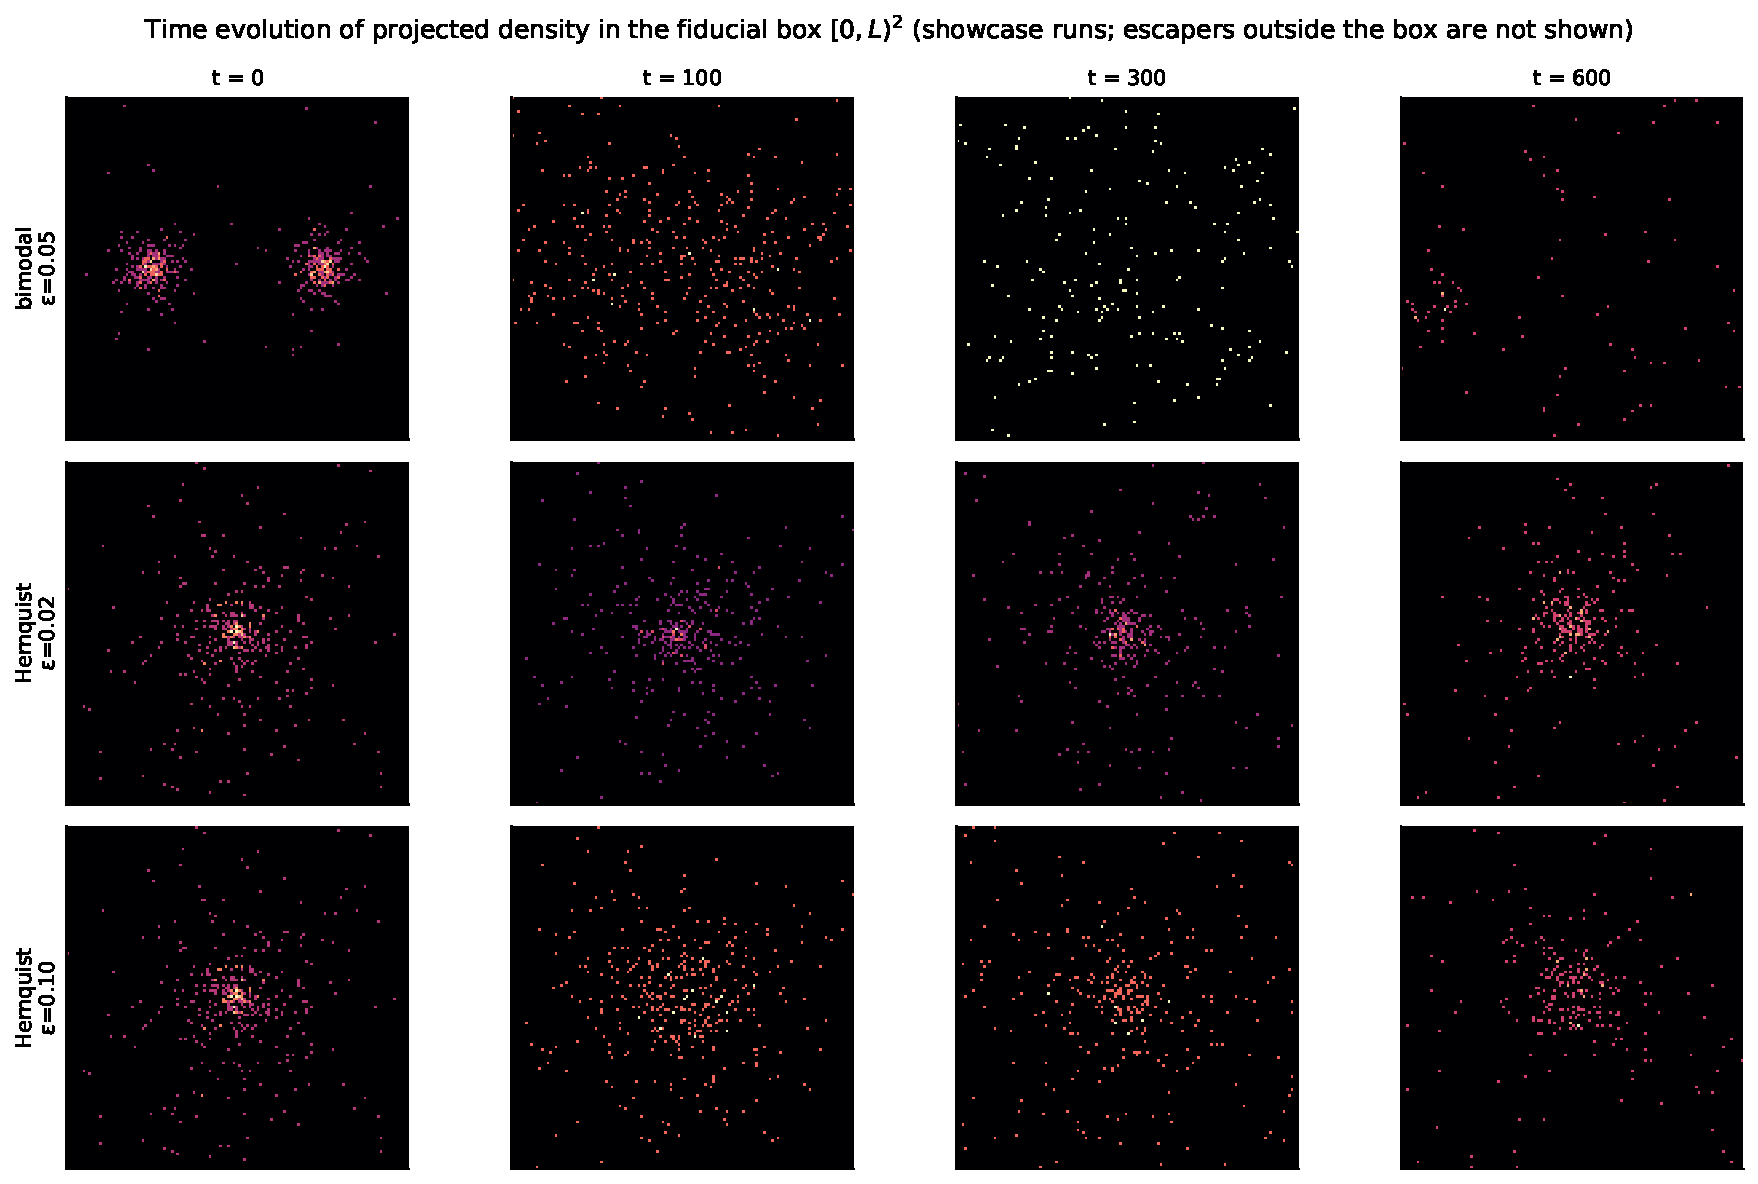
\includegraphics[width=\textwidth]{outputs/figures/fig02_snapshots.pdf}
\caption{Time evolution: projected density (log scale, $N = \ShowcaseN{}$,
  direct-isolated).
  \textit{Rows}: bimodal ($\heps = 0.05$); Hernquist ($\heps = 0.02$);
  Hernquist ($\heps = 0.10$).
  \textit{Columns}: $t = 0$, early, mid, final.
  The two Hernquist rows appear visually similar in projected density;
  the predictive difference between them is kinematic, not spatial
  (see Figure~\ref{fig:veldisp_mechanism}).}
\label{fig:snapshots}
\end{figure}

\subsection{Fine kinematic advantage at small softening}
\label{sec:results:cond_fine}

For concentrated profiles at small softening, the local velocity dispersion
shows the strongest fine signal in the battery.
Table~\ref{tab:cond_fine} shows VelDisp and kNN-all correlations across
all five softening values for Hernquist and Plummer at $N = 1024$.
For Hernquist at $\heps = 0.02$: $r_{\rm VD} = \HernquistVelDispR{}$
(95\% CI $[\HernquistVelDispCILo{}, \HernquistVelDispCIHi{}]$);
the kinematic gap CI is $[\HernquistKinGapCILo{}, \HernquistKinGapCIHi{}]$,
entirely above zero, confirming that VelDisp outperforms the best coarse
predictor at this softening.
For Plummer at $\heps = 0.02$: $r_{\rm VD} = \PlummerVelDispR{}$
(95\% CI $[\PlummerVelDispCILo{}, \PlummerVelDispCIHi{}]$),
also with a gap CI excluding zero.
The fine advantage erodes with increasing $\heps$: Hernquist reaches
a tie at $\heps = 0.07$ and coarse dominance at $\heps = 0.10$;
Plummer transitions to tie by $\heps = 0.03$ and coarse dominance by
$\heps = 0.07$.
\begin{table}[htbp]
\centering
\caption{VelDisp and kNN-all correlations across softening for
  Hernquist and Plummer at $N = 1024$, direct-isolated.
  VelDisp outperforms the coarse predictor at low $\heps$
  (gap CIs exclude zero for Hernquist at $\heps \le 0.05$ and
  Plummer at $\heps = 0.02$); kNN-all does not.}
\label{tab:cond_fine}
\begin{tabular}{llrrrrl}
\toprule
IC & $\epsilon$ & $r_{\rm VelDisp}$ & $r_{\rm kNN}$ & Pos.~gap CI & Kin.~gap CI & Verdict\\
\midrule
Hernquist & 0.02 & -0.430 & +0.370 & [+0.08, +0.19] & [+0.28, +0.53] & FINE\\
Hernquist & 0.03 & -0.437 & +0.332 & [+0.07, +0.21] & [+0.36, +0.59] & FINE\\
Hernquist & 0.05 & -0.459 & +0.177 & [-0.05, +0.19] & [+0.45, +0.66] & FINE\\
Hernquist & 0.07 & -0.434 & -0.162 & [-0.16, -0.08] & [+0.19, +0.40] & TIE\\
Hernquist & 0.10 & -0.364 & -0.582 & [-0.09, -0.04] & [-0.09, +0.10] & COARSE\\
\midrule
Plummer & 0.02 & -0.577 & +0.070 & [-0.37, -0.13] & [+0.41, +0.61] & FINE\\
Plummer & 0.03 & -0.566 & +0.005 & [-0.39, -0.23] & [+0.28, +0.49] & TIE\\
Plummer & 0.05 & -0.511 & -0.162 & [-0.37, -0.27] & [+0.09, +0.29] & TIE\\
Plummer & 0.07 & -0.431 & -0.499 & [-0.23, -0.16] & [-0.09, +0.09] & COARSE\\
Plummer & 0.10 & -0.318 & -0.736 & [-0.14, -0.08] & [-0.26, -0.09] & COARSE\\
\bottomrule
\end{tabular}

\end{table}

Figure~\ref{fig:cond_fine} shows how VelDisp, kNN-all, and CoarseG8
change with $\heps$ across the three families.
For concentrated profiles the VelDisp signal decays with increasing
$\heps$, reaching $r_{\rm VD} = \HernquistVelDispEpsTen{}$ for
Hernquist at $\heps = 0.10$.

\begin{figure}[htbp]
\centering
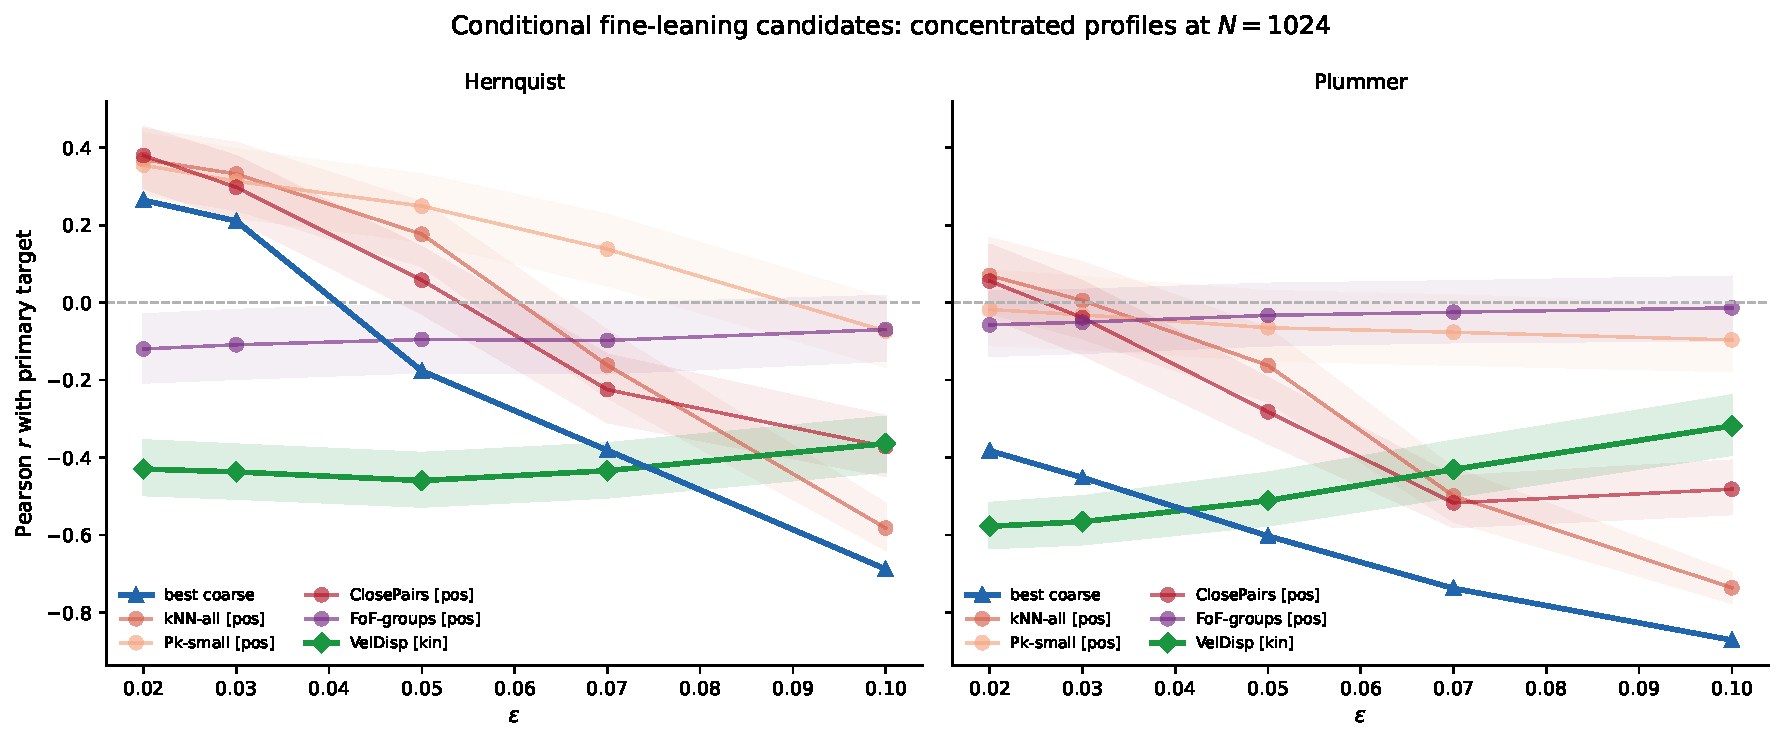
\includegraphics[width=\textwidth]{outputs/figures/fig05_cond_fine.pdf}
\caption{Observable class vs softening: $N = 1024$, direct-isolated.
  Solid: VelDisp (kinematic fine).
  Dashed: kNN-all (positional fine).
  Dotted: CoarseG8 (coarse).
  Shaded: 95\% bootstrap CI.
  VelDisp outperforms the coarse predictor at low $\heps$ for concentrated
  profiles; the advantage weakens with increasing $\heps$.
  kNN-all does not outperform the coarse predictor in any cell tested.}
\label{fig:cond_fine}
\end{figure}

Figure~\ref{fig:veldisp_mechanism} illustrates the softening dependence:
at $\heps = 0.02$ the velocity-dispersion map shows a concentrated hot
core; at $\heps = 0.10$ ($\heps/a \approx 0.5$) the cusp dynamics are
smoothed out and the kinematic signal disappears.

\begin{figure}[htbp]
\centering
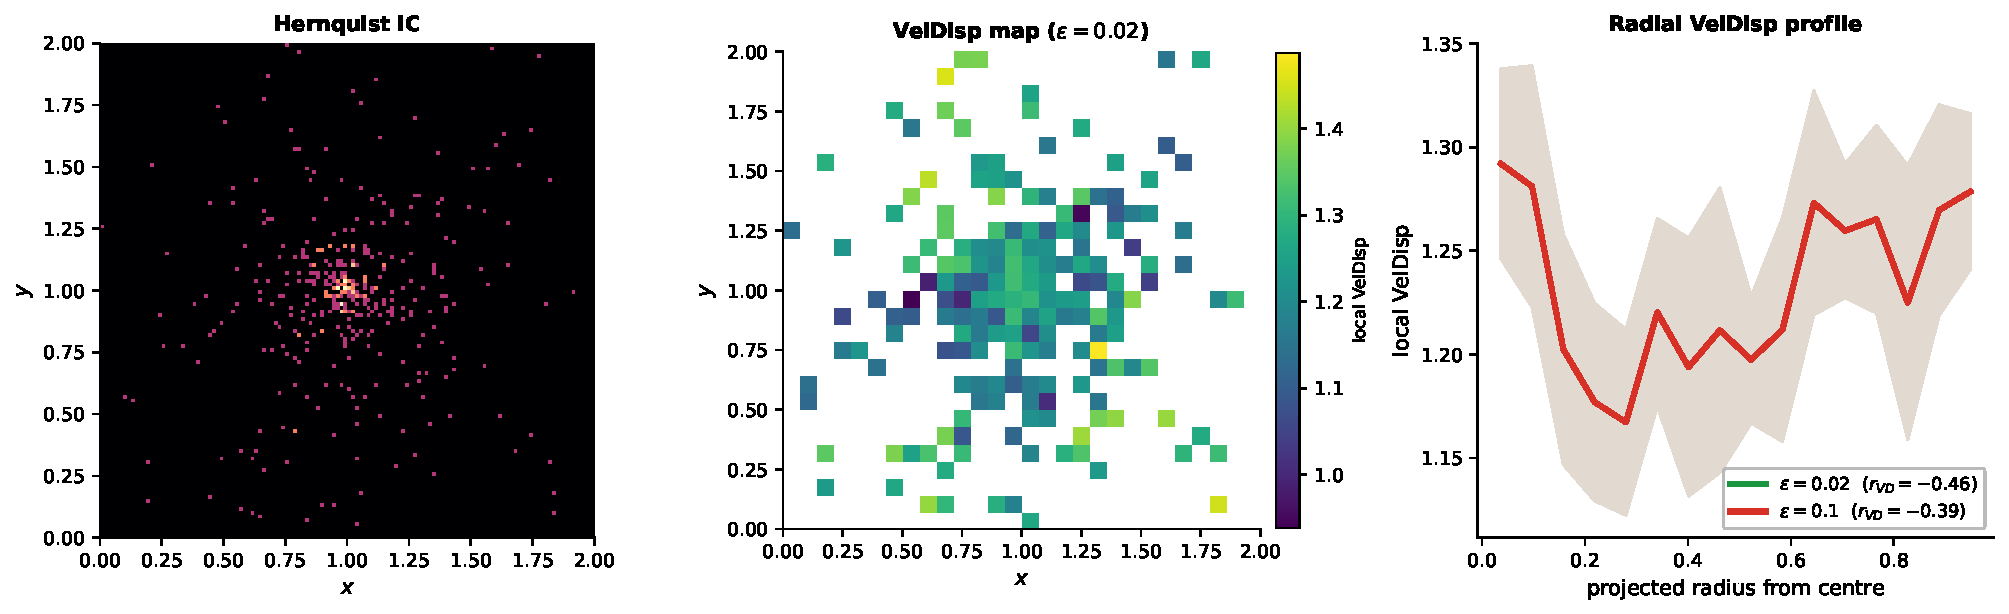
\includegraphics[width=\textwidth]{outputs/figures/fig12_veldisp_mechanism.pdf}
\caption{VelDisp mechanism: Hernquist profile at $N = \ShowcaseN{}$.
  \textit{Left}: projected particle density.
  \textit{Centre}: local velocity-dispersion map at $\heps = 0.02$.
  \textit{Right}: radial VelDisp profiles at $\heps = 0.02$ (green) and
  $\heps = 0.10$ (red), with $r$(VelDisp, $\dCearly$) annotated.
  The kinematic hot core is visible at small softening; at large softening
  the profile flattens and the predictive correlation weakens.}
\label{fig:veldisp_mechanism}
\end{figure}

\subsection{The softening transition}
\label{sec:results:eps_transition}

Figure~\ref{fig:eps_transition} shows for all four families how the
winner gap changes with $\heps$.

\begin{figure}[htbp]
\centering
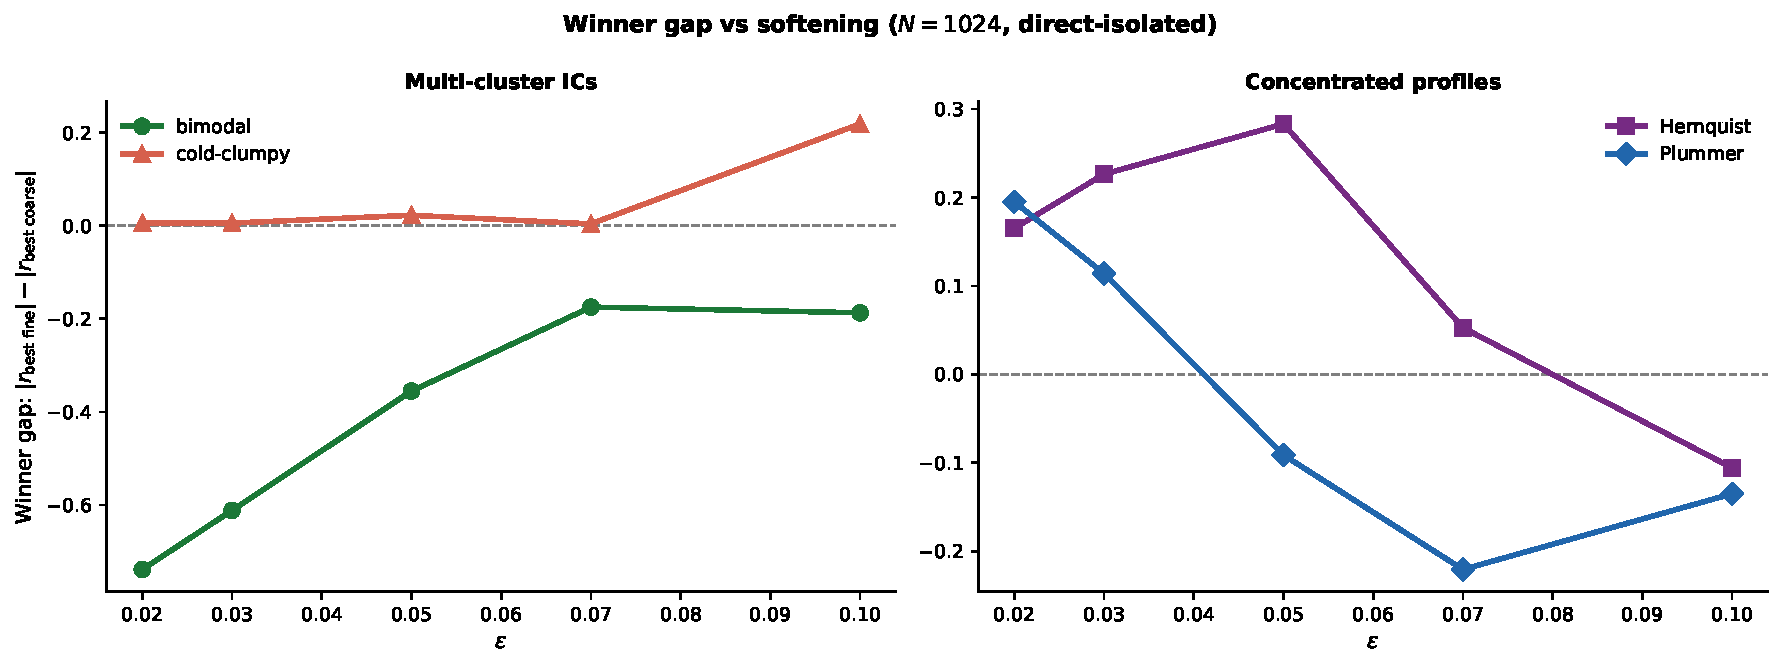
\includegraphics[width=\textwidth]{outputs/figures/fig06_eps_transition.pdf}
\caption{Winner gap vs softening: $N = 1024$, direct-isolated.
  Each curve shows the winner gap
  ($|r_{\rm best\,fine}| - |r_{\rm best\,coarse}|$; positive = fine advantage,
  negative = coarse dominance) for one IC family.
  Bimodal is strongly negative at all $\heps$.
  Concentrated profiles cross zero between $\heps = 0.05$ and $0.07$,
  transitioning from fine to coarse dominance.}
\label{fig:eps_transition}
\end{figure}

Bimodal remains strongly negative at all $\heps$ because the
dynamically decisive scale ($\sim 0.5\,L$) far exceeds the softening
length.  For Hernquist the winner gap crosses zero near
$\heps = 0.07$; Plummer crosses earlier.
The relevant ratio is $\heps/a$: the cusp is partially resolved at
$\heps/a = 0.10$ and smoothed out at $\heps/a = 0.50$.

Figure~\ref{fig:eps_boundary} plots the winner gap against
$\heps/a$.  The Hernquist zero-crossing occurs between
$\heps/a \approx 0.25$ and $0.50$; Plummer crosses earlier.
A finer $\heps/a$ sweep would locate the boundary more precisely.

\begin{figure}[htbp]
\centering
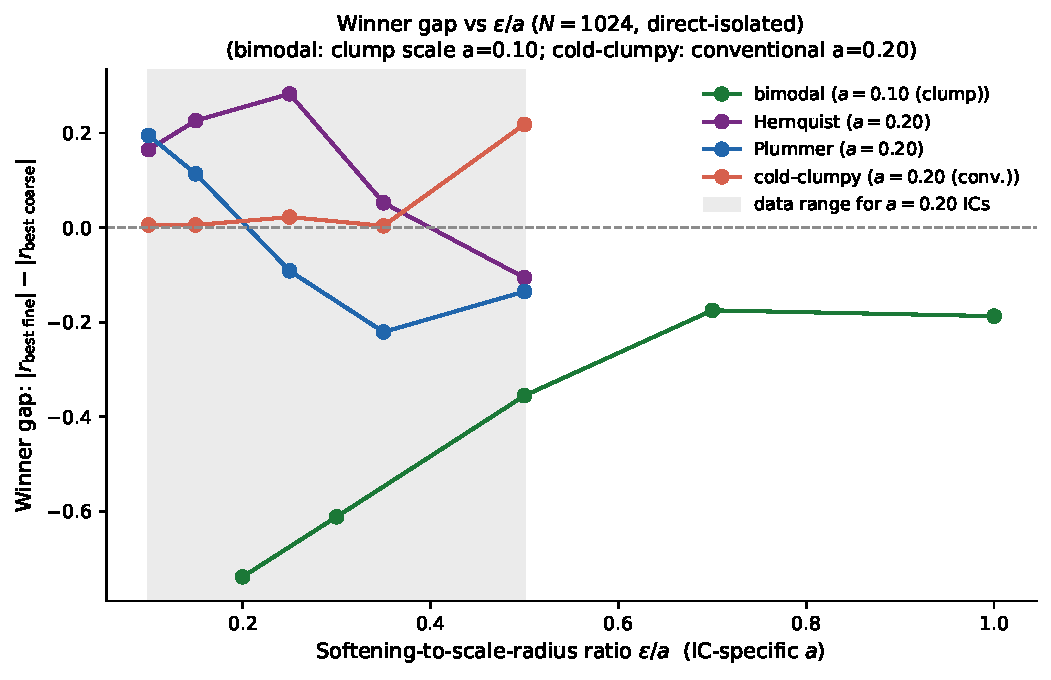
\includegraphics[width=0.72\textwidth]{outputs/figures/fig13_eps_boundary.pdf}
\caption{Verdict boundary in $\heps/a$: winner gap
  ($|r_{\rm best\,fine}| - |r_{\rm best\,coarse}|$) vs the
  softening-to-scale-radius ratio, $N = 1024$, direct-isolated.
  Each point is annotated with the verdict (C = \textsc{coarse},
  F = \textsc{fine}, T = tie).
  Bimodal is negative at all tested $\heps/a$.
  Hernquist and Plummer cross zero between $\heps/a \approx 0.15$ and
  $0.50$ (shaded zone), transitioning from fine to coarse dominance.}
\label{fig:eps_boundary}
\end{figure}

\subsection{N-scaling}
\label{sec:results:n_scaling}

Figure~\ref{fig:n_scaling} shows $r_{\rm CG8}$ and the best fine predictor
vs $N$ for all four families, at each $\heps$ value.

\begin{figure}[htbp]
\centering
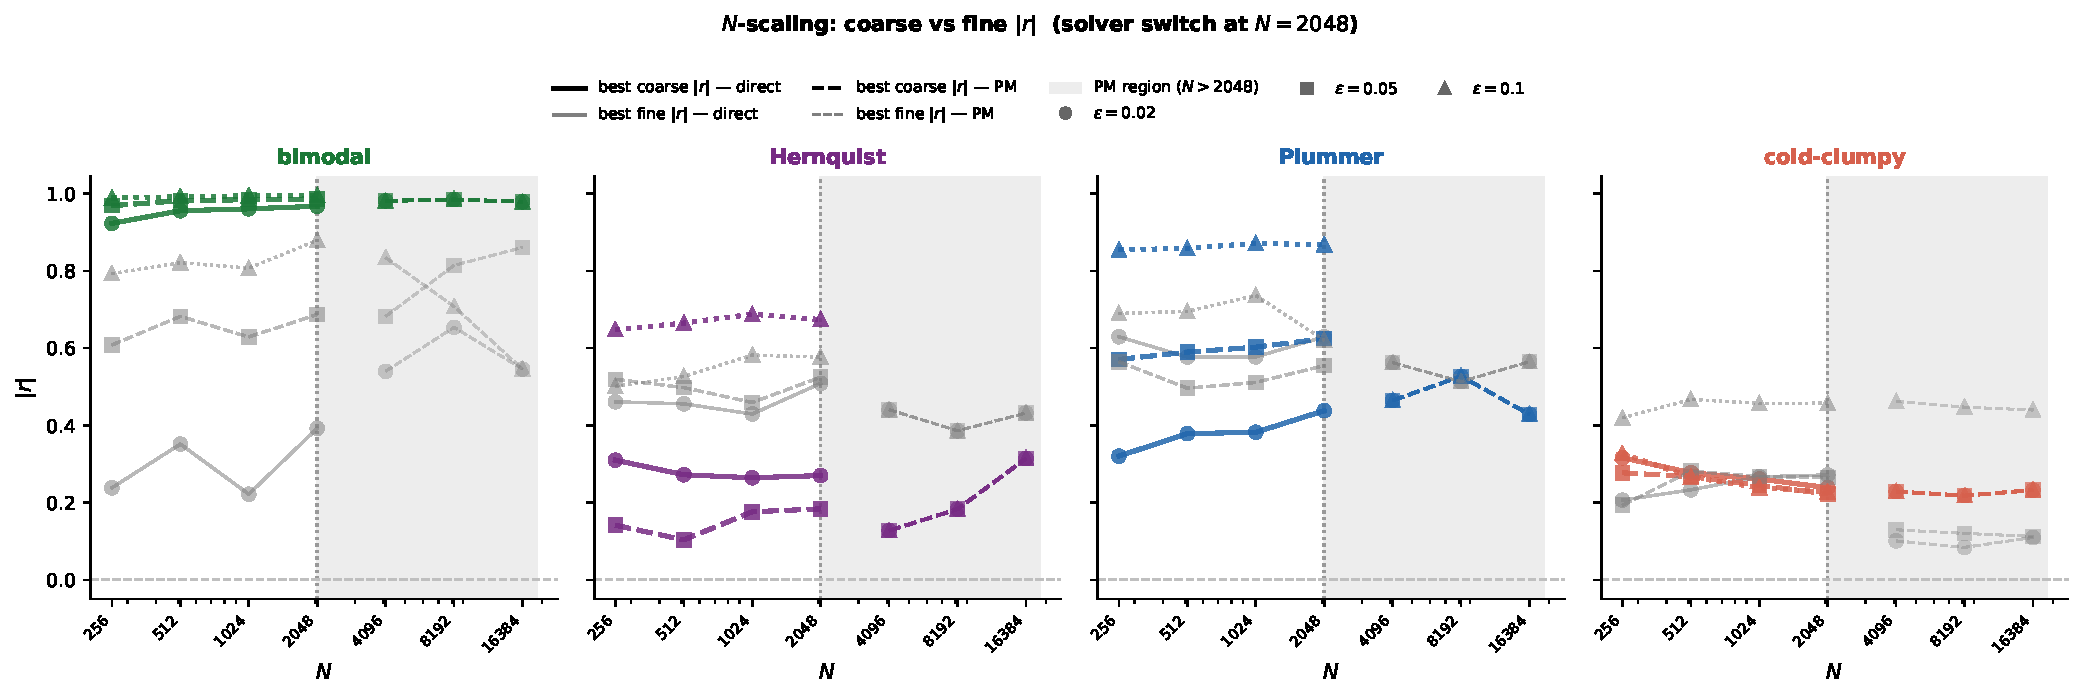
\includegraphics[width=\textwidth]{outputs/figures/fig07_n_scaling.pdf}
\caption{N-scaling at three softening values, direct-isolated.
  Each panel: one IC family.
  Coloured lines: $r_{\rm CG8}$ (solid/dashed/dotted for
  $\heps = 0.02/0.05/0.10$).
  Grey: best fine predictor.
  Bimodal is stable near $-0.98$ at all $N$ and $\heps$.}
\label{fig:n_scaling}
\end{figure}

The bimodal verdict is stable across $N$ at all $\heps$.
For concentrated profiles, VelDisp improves modestly with $N$ and the
fine advantage at small $\heps$ persists; no verdict reversal occurs.

\subsection{Force-model comparison}
\label{sec:results:model_compare}

Figure~\ref{fig:model_comparison} shows $r_{\rm CG8}$ vs $\heps$ for
both model classes at $N = 1024$.

\begin{figure}[htbp]
\centering
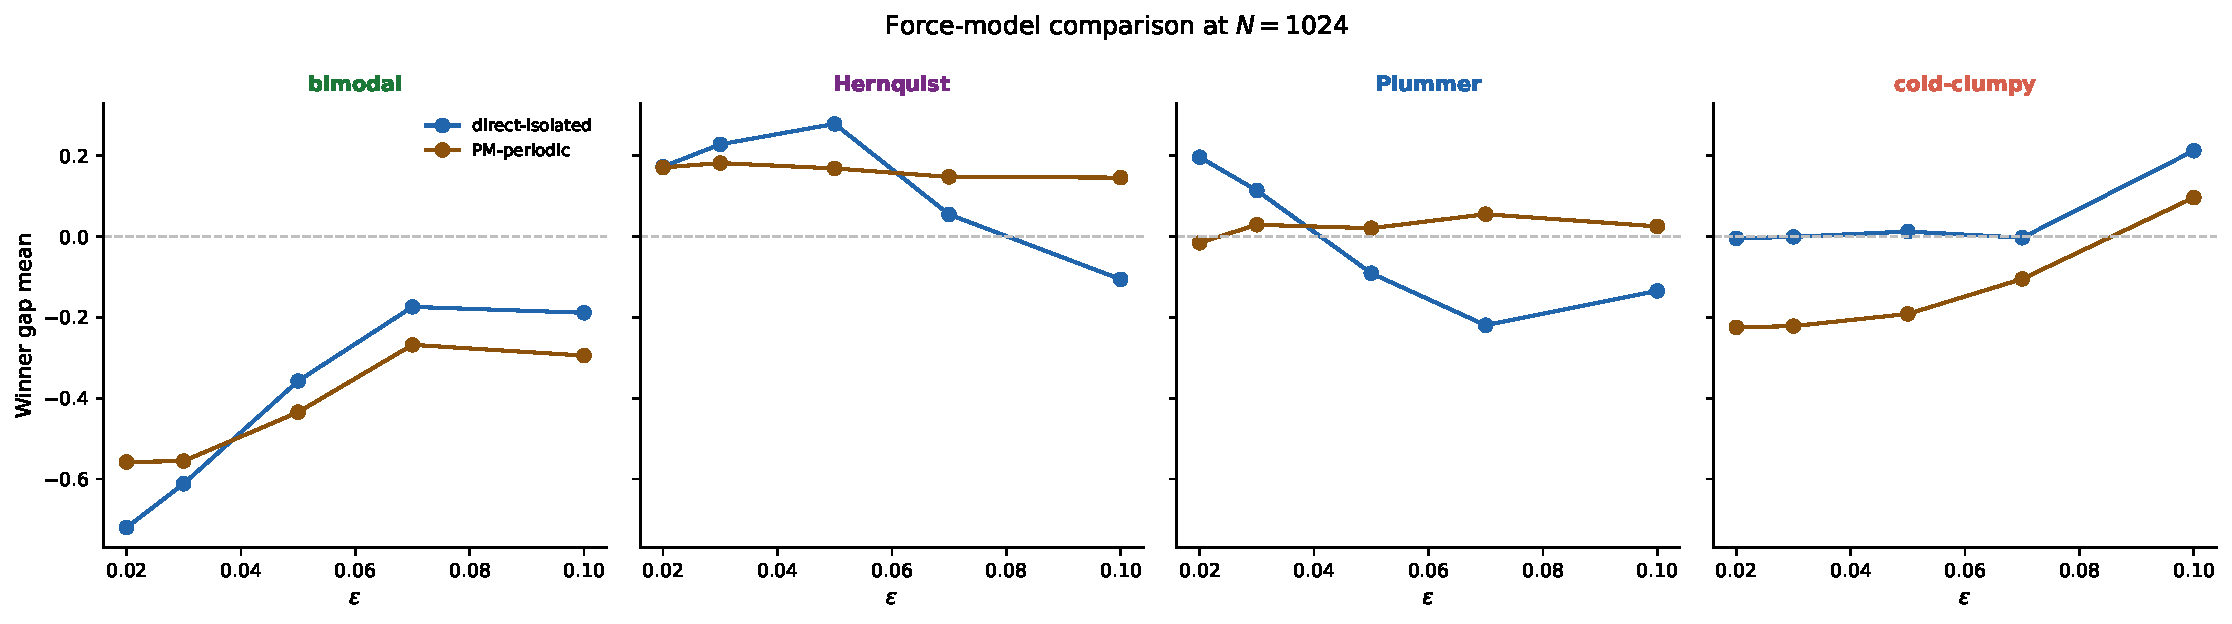
\includegraphics[width=\textwidth]{outputs/figures/fig08_model_comparison.pdf}
\caption{Force-model comparison: $r_{\rm CG8}$ vs $\heps$, $N = 1024$.
  Blue: direct-isolated.  Brown: PM-periodic.
  Shaded: 95\% CI.
  Both models agree on the bimodal verdict.
  Concentrated profiles show quantitative differences: direct-isolated
  exhibits a clear $\heps$-dependent transition while PM-periodic is
  nearly $\heps$-invariant (force resolution set by grid, not $\heps$).}
\label{fig:model_comparison}
\end{figure}

Both model classes agree on the bimodal verdict at all $\heps$.
For concentrated profiles, quantitative differences arise because the
PM force resolution ($\sim L/32$) is set by the mesh, making PM rows
nearly $\heps$-invariant.  The direct-isolated results show the
clearest $\heps$-dependent transition.

\subsection{Observable-class dependence}
\label{sec:results:obs_class}

The main verdict table (Table~\ref{tab:verdict_summary}) summarises
verdicts across both force-model classes, all initial-condition families,
and all softening values at $N = 1024$.

\begin{table}[htbp]
\centering
\caption{Verdict summary at $N = 1024$, both force-model classes,
  all initial-condition families, and $\heps \in \{0.02, 0.03, 0.05, 0.07, 0.10\}$.
  Gap column shows $|r_{\rm best\,fine}| - |r_{\rm best\,coarse}|$.}
\label{tab:verdict_summary}
\resizebox{\textwidth}{!}{%
\begin{tabular}{lllrrrrrrlr}
\toprule
Model & IC & $\epsilon$ & Best coarse & $|r|_{\rm bc}$ & Best fine & $|r|_{\rm bf}$ & Gap mean & Gap CI & Verdict & $n_{\rm lw}$\\
\midrule
direct-isolated & bimodal & 0.02 & CoarseG8 & +0.961 & ClosePairs & +0.222 & -0.720 & [-0.78, -0.65] & COARSE & 500\\
direct-isolated & bimodal & 0.03 & CoarseG8 & +0.972 & ClosePairs & +0.360 & -0.611 & [-0.69, -0.53] & COARSE & 500\\
direct-isolated & bimodal & 0.05 & CoarseG8 & +0.984 & ClosePairs & +0.629 & -0.357 & [-0.42, -0.30] & COARSE & 500\\
direct-isolated & bimodal & 0.07 & CoarseG8 & +0.990 & ClosePairs & +0.815 & -0.174 & [-0.21, -0.14] & COARSE & 500\\
direct-isolated & bimodal & 0.10 & CoarseG8 & +0.994 & kNN-all & +0.807 & -0.189 & [-0.22, -0.16] & COARSE & 500\\
direct-isolated & Hernquist & 0.02 & CoarseG16 & +0.264 & VelDisp & +0.430 & +0.172 & [+0.09, +0.28] & FINE & 500\\
direct-isolated & Hernquist & 0.03 & CoarseG16 & +0.211 & VelDisp & +0.437 & +0.228 & [+0.12, +0.34] & FINE & 500\\
direct-isolated & Hernquist & 0.05 & CoarseG8 & +0.176 & VelDisp & +0.459 & +0.278 & [+0.17, +0.38] & FINE & 500\\
direct-isolated & Hernquist & 0.07 & CoarseG8 & +0.381 & VelDisp & +0.434 & +0.054 & [-0.05, +0.16] & TIE & 500\\
direct-isolated & Hernquist & 0.10 & CoarseG8 & +0.688 & kNN-all & +0.582 & -0.106 & [-0.13, -0.08] & COARSE & 500\\
direct-isolated & Plummer & 0.02 & CoarseG8 & +0.382 & VelDisp & +0.577 & +0.196 & [+0.09, +0.30] & FINE & 500\\
direct-isolated & Plummer & 0.03 & CoarseG8 & +0.452 & VelDisp & +0.566 & +0.113 & [+0.01, +0.22] & TIE & 500\\
direct-isolated & Plummer & 0.05 & CoarseG8 & +0.603 & VelDisp & +0.511 & -0.091 & [-0.18, +0.01] & TIE & 500\\
direct-isolated & Plummer & 0.07 & CoarseG8 & +0.738 & ClosePairs & +0.517 & -0.220 & [-0.26, -0.18] & COARSE & 500\\
direct-isolated & Plummer & 0.10 & CoarseG8 & +0.871 & kNN-all & +0.736 & -0.135 & [-0.16, -0.11] & COARSE & 500\\
direct-isolated & cold-clumpy & 0.02 & CoarseG8 & +0.261 & FoF-groups & +0.267 & -0.005 & [-0.14, +0.13] & TIE & 500\\
direct-isolated & cold-clumpy & 0.03 & CoarseG8 & +0.257 & FoF-groups & +0.262 & -0.001 & [-0.15, +0.14] & TIE & 500\\
direct-isolated & cold-clumpy & 0.05 & CoarseG8 & +0.245 & FoF-groups & +0.268 & +0.012 & [-0.15, +0.17] & TIE & 500\\
direct-isolated & cold-clumpy & 0.07 & CoarseG8 & +0.239 & FoF-groups & +0.243 & -0.003 & [-0.14, +0.14] & TIE & 500\\
direct-isolated & cold-clumpy & 0.10 & CoarseG8 & +0.239 & ClosePairs & +0.457 & +0.212 & [+0.10, +0.31] & FINE & 500\\
\midrule
PM-periodic & bimodal & 0.02 & CoarseG8 & +0.978 & FoF-groups & +0.568 & -0.558 & [-0.62, -0.50] & COARSE & 500\\
PM-periodic & bimodal & 0.03 & CoarseG8 & +0.978 & FoF-groups & +0.568 & -0.555 & [-0.62, -0.50] & COARSE & 500\\
PM-periodic & bimodal & 0.05 & CoarseG8 & +0.978 & ClosePairs & +0.612 & -0.435 & [-0.49, -0.38] & COARSE & 500\\
PM-periodic & bimodal & 0.07 & CoarseG8 & +0.978 & ClosePairs & +0.793 & -0.268 & [-0.30, -0.23] & COARSE & 500\\
PM-periodic & bimodal & 0.10 & CoarseG8 & +0.978 & kNN-all & +0.784 & -0.295 & [-0.33, -0.26] & COARSE & 500\\
PM-periodic & Hernquist & 0.02 & CoarseG16 & +0.239 & VelDisp & +0.453 & +0.170 & [+0.07, +0.28] & FINE & 500\\
PM-periodic & Hernquist & 0.03 & CoarseG16 & +0.239 & VelDisp & +0.453 & +0.181 & [+0.07, +0.29] & FINE & 500\\
PM-periodic & Hernquist & 0.05 & CoarseG16 & +0.239 & VelDisp & +0.453 & +0.168 & [+0.05, +0.28] & FINE & 500\\
PM-periodic & Hernquist & 0.07 & CoarseG16 & +0.239 & VelDisp & +0.453 & +0.147 & [+0.03, +0.27] & TIE & 500\\
PM-periodic & Hernquist & 0.10 & CoarseG16 & +0.239 & VelDisp & +0.453 & +0.145 & [+0.03, +0.27] & TIE & 500\\
PM-periodic & Plummer & 0.02 & CoarseG8 & +0.451 & VelDisp & +0.563 & -0.016 & [-0.11, +0.09] & TIE & 500\\
PM-periodic & Plummer & 0.03 & CoarseG8 & +0.451 & VelDisp & +0.563 & +0.029 & [-0.07, +0.13] & TIE & 500\\
PM-periodic & Plummer & 0.05 & CoarseG8 & +0.451 & VelDisp & +0.563 & +0.020 & [-0.09, +0.13] & TIE & 500\\
PM-periodic & Plummer & 0.07 & CoarseG8 & +0.451 & VelDisp & +0.563 & +0.055 & [-0.04, +0.15] & TIE & 500\\
PM-periodic & Plummer & 0.10 & CoarseG8 & +0.451 & VelDisp & +0.563 & +0.025 & [-0.07, +0.13] & TIE & 500\\
PM-periodic & cold-clumpy & 0.02 & CoarseG8 & +0.248 & ClosePairs & +0.037 & -0.225 & [-0.31, -0.12] & COARSE & 500\\
PM-periodic & cold-clumpy & 0.03 & CoarseG8 & +0.248 & ClosePairs & +0.038 & -0.222 & [-0.31, -0.12] & COARSE & 500\\
PM-periodic & cold-clumpy & 0.05 & CoarseG8 & +0.248 & ClosePairs & +0.086 & -0.192 & [-0.31, -0.06] & COARSE & 500\\
PM-periodic & cold-clumpy & 0.07 & CoarseG8 & +0.248 & ClosePairs & +0.191 & -0.105 & [-0.25, +0.03] & TIE & 500\\
PM-periodic & cold-clumpy & 0.10 & CoarseG8 & +0.248 & ClosePairs & +0.449 & +0.096 & [-0.04, +0.21] & TIE & 500\\
\bottomrule
\end{tabular}

}
\end{table}

Three patterns hold: (i) no positional fine observable outperforms the
coarse predictor in any cell; (ii) FoF group count never outperforms
the coarse predictor (it may appear as ``best fine'' in some cells of
Table~\ref{tab:verdict_summary}, meaning only that it is the
least-weak fine observable, not that it outperforms coarse);
(iii) VelDisp is the only fine observable whose gap CIs
exclude zero, and only for concentrated profiles at small $\heps$.
The cold-clumpy family shows a single anomalous \textsc{fine} verdict at
$\heps = 0.10$ (Table~\ref{tab:verdict_summary}), driven by the
ClosePairs observable.  At large softening, the linking radius
$4\heps = 0.40$ approaches the inter-clump separation, making ClosePairs
a proxy for inter-clump connectivity rather than true fine-scale
structure.  This cell does not reflect a physical fine-scale advantage.

\subsection{Summary matrix}
\label{sec:results:summary}

Figure~\ref{fig:summary_matrix} shows $r$ for all observable class
$\times$ $\heps$ combinations as a colour matrix.

\begin{figure}[htbp]
\centering
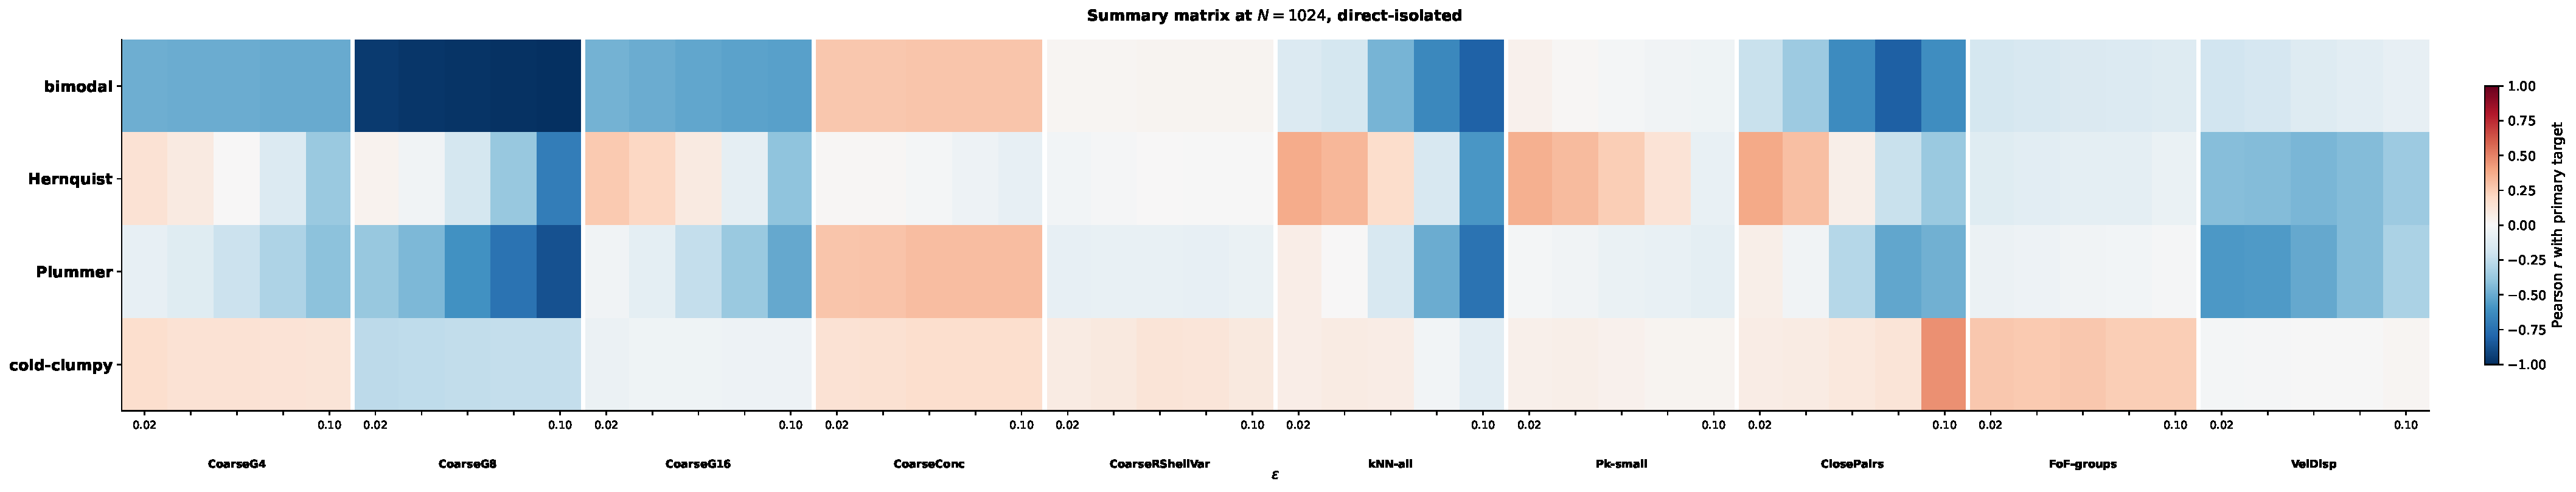
\includegraphics[width=\textwidth]{outputs/figures/fig10_summary_matrix.pdf}
\caption{Summary matrix: Pearson $r$ with $\dCearly$ by IC family (rows),
  observable class (groups), and $\heps$ (within-group columns),
  at $N = 1024$, direct-isolated.
  The coarse group (leftmost) shows strong negative $r$ for bimodal at all
  $\heps$.
  VelDisp (fine kinematic) shows the strongest fine signal for Hernquist and
  Plummer at $\heps = 0.02$.
  No tested positional fine observable outperforms the coarse predictor
  in any cell.}
\label{fig:summary_matrix}
\end{figure}

Figure~\ref{fig:class_gap} summarises the gap structure at the
observable-class level, showing that the kinematic fine class produces
the only gaps that exclude zero against the coarse predictor, while
positional fine classes do not.

\begin{figure}[htbp]
\centering
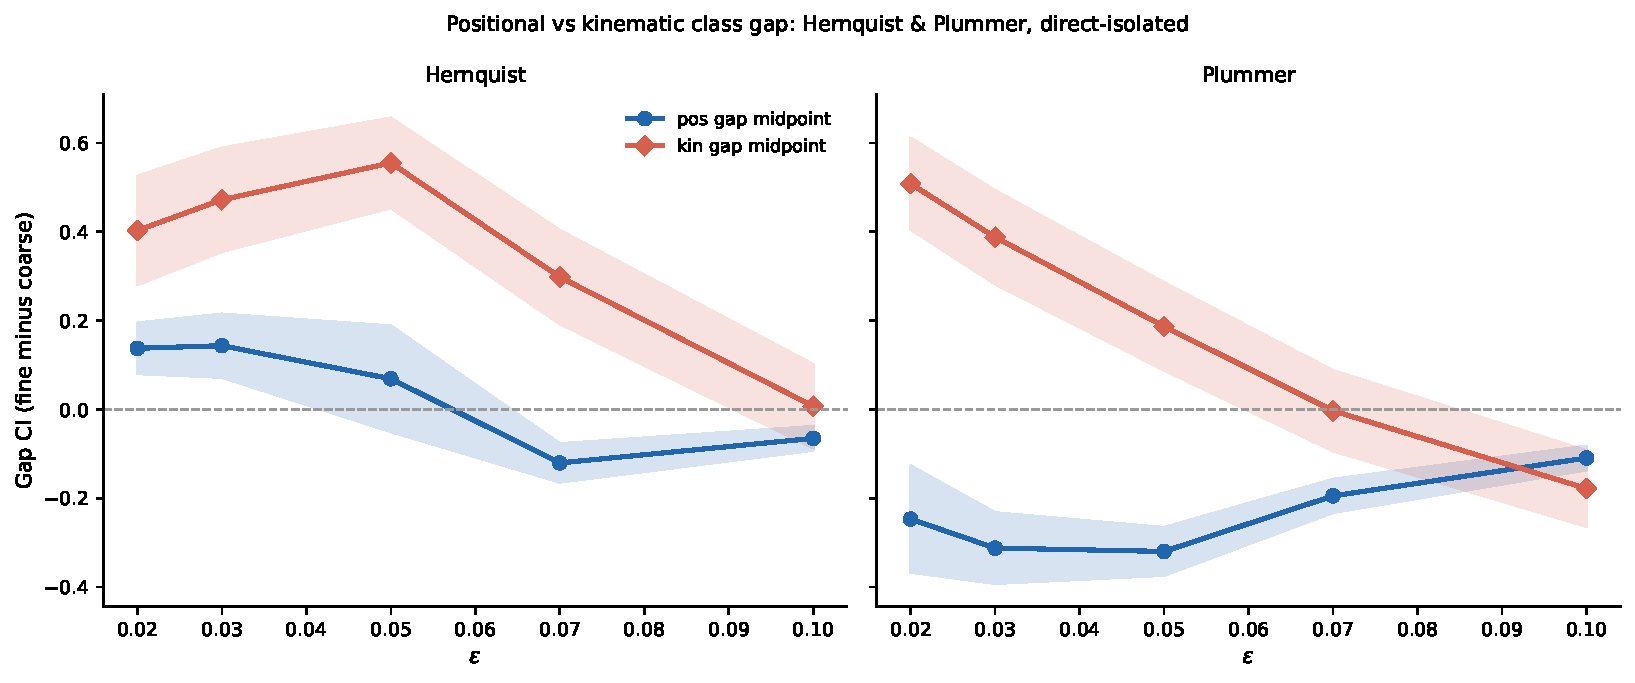
\includegraphics[width=\textwidth]{outputs/figures/fig15_class_gap.pdf}
\caption{Class-level gap summary: distribution of
  $|r_{\rm fine}| - |r_{\rm coarse}|$ grouped by observable class
  (positional fine, kinematic fine) across all IC families and
  $\heps$ values at $N = 1024$, direct-isolated.
  Kinematic fine (VelDisp) is the only class whose gap distribution
  extends above zero for concentrated profiles at low $\heps$.
  Positional fine classes remain below or near zero in all tested cells.}
\label{fig:class_gap}
\end{figure}
% SUPPLEMENTARY CANDIDATE: Fig 15 (class-level gap) could move to appendix.

The matrix confirms the observable-class structure: coarse dominates for
bimodal at all $\heps$, VelDisp shows a fine advantage for concentrated
profiles at low $\heps$ only, and no positional fine observable exceeds
the coarse predictor in any cell.


% ---------------------------------------------------------------------------
\section{Discussion}
\label{sec:discussion}

\subsection{Physical interpretation: bimodal case}

In a two-cluster merger the dominant dynamical variable is the inter-cluster
density contrast, encoded in $\sigrho(8)$ at grid scale $L/8 \approx 0.25$.
The merger timescale $t_{\rm merge} \sim d/v_{\rm rel}$ depends on
large-scale quantities; realisations with higher initial contrast merge
faster and produce more clustering growth by the early horizon.
Sub-cluster internal structure is dynamically decoupled at early times,
explaining why positional fine observables carry no additional predictive
power.

\subsection{Physical interpretation: concentrated profiles}

Local velocity dispersion encodes kinematic pressure: regions with
higher initial $\sigma_v^{\rm loc}$ have more virial support and resist
collapse, producing a negative correlation with future clustering growth.
Positional fine observables cannot detect this because the equilibrium
density profile is smooth above the softening scale; the fine advantage
is observable-class-specific, requiring phase-space access.

Increasing $\heps$ smooths the potential over scales comparable to the
cusp radius $a$.  The transition from fine to coarse dominance lies
between $\heps/a \approx 0.25$ and $0.50$ for Hernquist, and at lower
$\heps/a$ for Plummer.  The five-point grid resolves the direction but
not the precise boundary.

Figure~\ref{fig:radial_and_null} shows that the main predictive signals
are not trivially explained by radial distance from the cluster centre
or by null-shuffled controls, arguing against the simplest radial
and permutation-null explanations.

\begin{figure}[htbp]
\centering
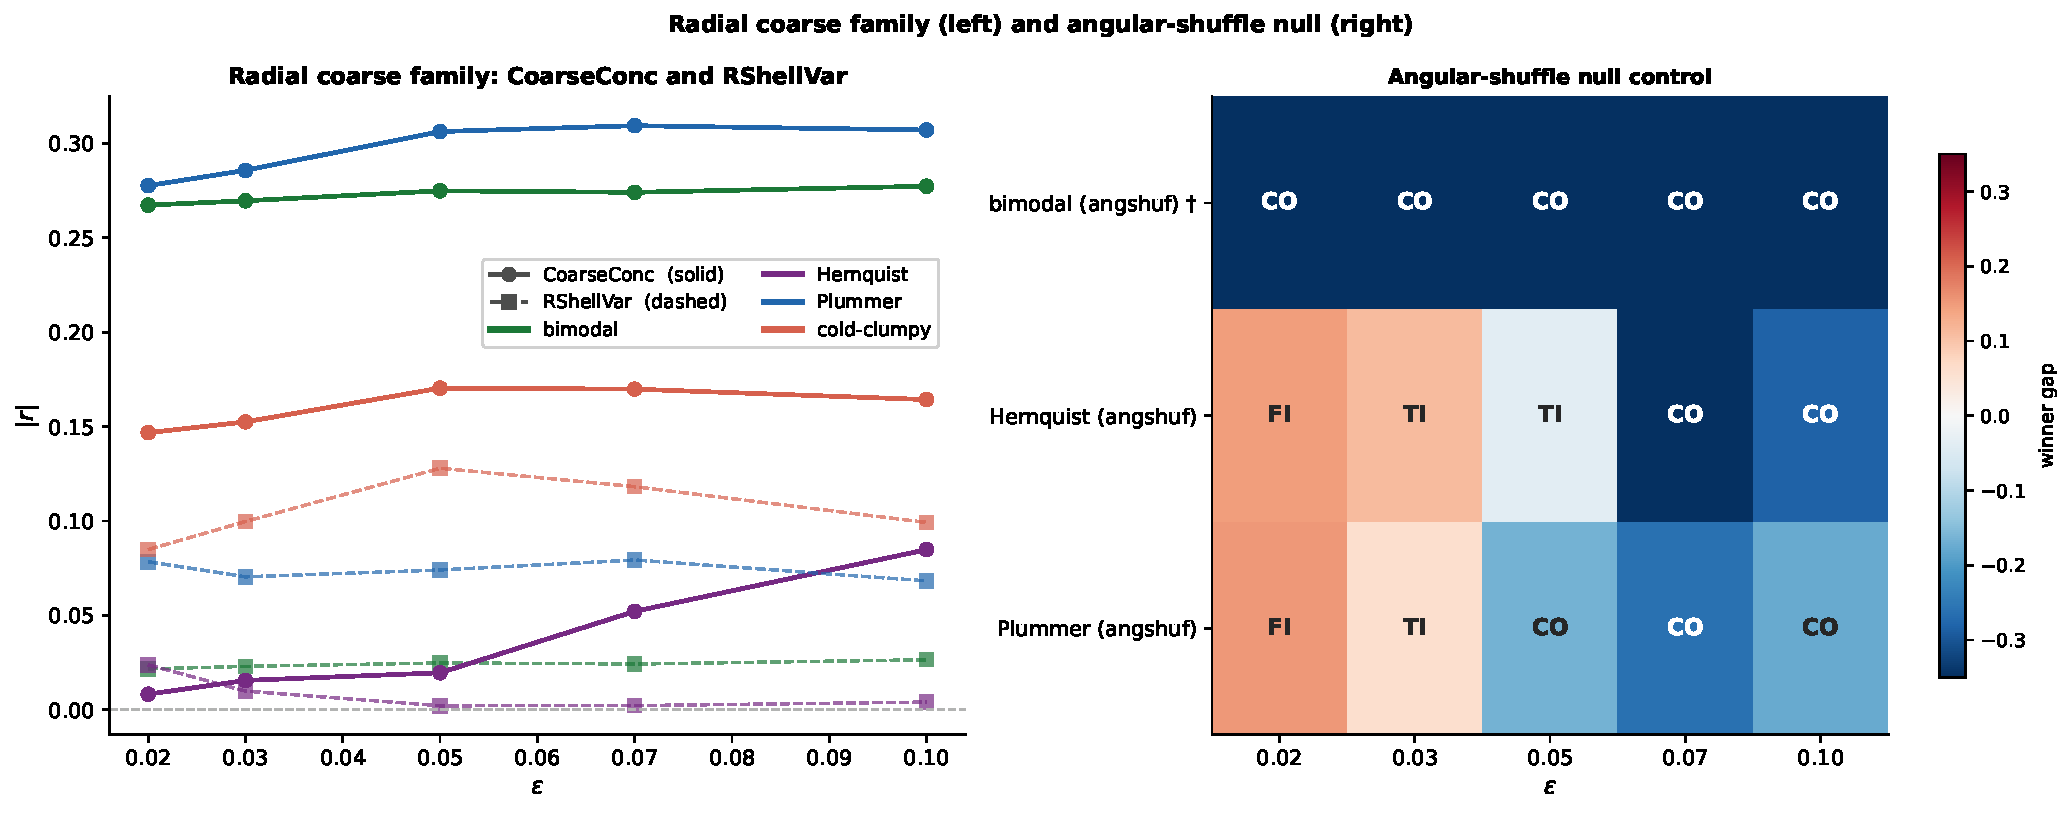
\includegraphics[width=\textwidth]{outputs/figures/fig17_radial_and_null.pdf}
\caption{Diagnostic controls.
  \textit{Left}: predictive correlation of the radial-distance summary
  vs the primary coarse and fine observables; radial distance alone
  does not account for the observed gaps.
  \textit{Right}: null-shuffled controls in which observable--outcome
  pairs are randomly permuted; shuffled correlations are centred on
  zero, confirming that the reported signals are not statistical
  artefacts.}
\label{fig:radial_and_null}
\end{figure}
% SUPPLEMENTARY CANDIDATE: Fig 17 (radial/null controls) could move to appendix.

\subsection{Astrophysical implications}

The bimodal merger timescale $t_{\rm merge} \sim d/v_{\rm rel}$ is
analogous to the dynamical friction timescale in galaxy mergers, and
the coarse density variance at scale $L/8$ measures essentially the
large-scale overdensity that drives dynamical friction.  For dark matter
halo mergers, this is consistent with the picture that the large-scale
density contrast at the virial-radius scale, not internal substructure,
governs the merger rate---as assumed in merger-tree models used in
cosmological simulations \citep{NFW1996}.

The $\heps/a$ transition maps onto whether a simulation resolves the
half-mass radius of a cusp.  For dark matter haloes with NFW-like cusps
($r_s \sim 10$--$30$~kpc), the critical softening implied by our results
is $\heps \sim 0.25\,r_s$.  Below this threshold, velocity-dispersion
substructure carries predictive information about future collapse;
above it, the kinematic signal vanishes.  This is consistent with the
\citet{PowerEtal2003} convergence criterion, which requires force
resolution well inside the scale radius for reliable halo profiles.

Self-gravitating $N$-body systems are the fundamental building blocks of
dark matter structure formation.  The finding that coarse density
contrast dominates prediction for multi-component mergers is consistent
with the hierarchical merging picture, where large-scale overdensity
determines collapse timing.  The kinematic fine advantage for
concentrated cusps suggests that velocity anisotropy and phase-space
substructure (streams, shells) may carry predictive information in
resolved dark matter haloes---connecting to debates on the diagnostic
role of internal kinematics in the cusp--core and missing-satellites
problems.

These results have practical implications for $N$-body simulation design.
For simulations of merging systems (galaxy pairs, halo mergers), the
coarse density field at the virial-radius scale is the primary predictor
of merger outcome; initial substructure below this scale is dynamically
irrelevant at early times.  For simulations of isolated cusp-dominated
systems (elliptical galaxies, dark matter haloes), force resolution must
satisfy $\heps/a \lesssim 0.25$ for initial velocity substructure to
carry predictive information.  Above this threshold, the kinematic signal
vanishes and only the coarse density field matters.

\subsection{What is and is not earned}
\label{sec:discussion:scope}

\textit{Earned.}  Bimodal coarse dominance holds across all tested $N$,
$\heps$, and force models.  No positional fine observable outperforms the
coarse predictor in any cell.  VelDisp outperforms it for concentrated
profiles at low softening (gap CIs exclude zero), with a real
$\heps$-dependent transition governed in part by $\heps/a$.

\textit{Unresolved.}  Hernquist at $\heps = 0.07$ and Plummer at
$\heps = 0.03$--$0.05$ have gap CIs spanning zero.  The precise
transition $\heps/a$ is not sharply located.

\textit{Not earned.}  Universal coarse dominance, universal fine
superiority, or a sharp critical boundary in $\heps/a$.  Family
stability is low (43 of \NCells{} powered cells spanning all $N$,
$\heps$, and both models), so a stable law across
families is not supported.  The study measures correlation, not
causation, and excludes cosmological processes.

\subsection{Scope and limitations}

The prediction target is a single scalar ($\dCearly$); fine observables
might carry more information for spatially resolved targets or longer
horizons.  The five-point $\heps$ grid resolves transition direction
but not the precise boundary in $\heps/a$.


% ---------------------------------------------------------------------------
\section{Conclusion}
\label{sec:conclusion}

Across \TotalRuns{} simulations spanning \NICs{} initial-condition
families, \NModels{} force models, and $\heps \in [\EpsMin{}, \EpsMax{}]$,
the central result is a verdict asymmetry between observable classes.
Bimodal (two-cluster) initial conditions are coarse-dominant in every
tested cell---all $N$, $\heps$, and both force models---with
$r = \BimodalBestCoarseR{}$ and a winner-gap CI entirely below zero.
For concentrated profiles (Hernquist, Plummer), local velocity dispersion
outperforms the coarse predictor at low softening ($\heps \le 0.05$ for
Hernquist, $\heps = 0.02$ for Plummer), with a transition to coarse
dominance by $\heps = 0.10$.
No tested positional fine observable outperforms the coarse predictor
in any parameter cell.  The kinematic fine advantage requires three
conditions simultaneously: a concentrated-cusp family, small $\heps/a$,
and phase-space access.
Outside this intersection, coarse dominance or ties prevail.

\clearpage

\section*{Data and Code Availability}

All simulation code, analysis pipeline, figure generation, and regression
tests are publicly available at
\url{https://github.com/kunalb541/NBODY}.
The repository includes:
\texttt{nbody\_stress.py} (battery runner and statistical analysis),
\texttt{nbody\_paper.py} (figure and table generation),
\texttt{nbody\_3d.py} (force models and integrators),
\texttt{test\_regression.py} (34 regression tests), and
\texttt{build.sh} (reproducible build script).
The full \TotalRuns{}-run battery CSV ($\sim 53$\,MB) is not included in
the repository but can be regenerated from scratch using
\texttt{python nbody\_paper.py --workers 30} (approximately 28~hours on
32~vCPUs) or reproduced via \texttt{--resume} for incremental runs.
Pre-computed figures and tables are included in \texttt{outputs/}.

\clearpage

\begin{thebibliography}{99}

\bibitem[Binney \& Tremaine(2008)]{BinneyTremaine2008}
Binney, J., \& Tremaine, S.\ 2008, \textit{Galactic Dynamics}, 2nd ed.,
Princeton University Press.

\bibitem[Hernquist(1990)]{Hernquist1990}
Hernquist, L.\ 1990, \textit{Astrophysical Journal}, 356, 359.

\bibitem[Hockney \& Eastwood(1988)]{HockneyEastwood1988}
Hockney, R.~W., \& Eastwood, J.~W.\ 1988,
\textit{Computer Simulation Using Particles}, Taylor \& Francis.

\bibitem[Plummer(1911)]{Plummer1911}
Plummer, H.~C.\ 1911,
\textit{Monthly Notices of the Royal Astronomical Society}, 71, 460.

\bibitem[Power et al.(2003)]{PowerEtal2003}
Power, C., Navarro, J.~F., Jenkins, A., et al.\ 2003,
\textit{Monthly Notices of the Royal Astronomical Society}, 338, 14.

\bibitem[Quinn et al.(1997)]{Quinn1997}
Quinn, T., Katz, N., Stadel, J., \& Lake, G.\ 1997,
arXiv:astro-ph/9710043.

\bibitem[Yoshida(1990)]{Yoshida1990}
Yoshida, H.\ 1990, \textit{Physics Letters A}, 150, 262.

\bibitem[Navarro et al.(1996)]{NFW1996}
Navarro, J.~F., Frenk, C.~S., \& White, S.~D.~M.\ 1996,
\textit{Astrophysical Journal}, 462, 563.

\bibitem[Navarro et al.(1997)]{NFW1997}
Navarro, J.~F., Frenk, C.~S., \& White, S.~D.~M.\ 1997,
\textit{Astrophysical Journal}, 490, 493.

\end{thebibliography}

\end{document}
